% Generated by Sphinx.
\def\sphinxdocclass{report}
\documentclass[a4,10pt,french]{sphinxmanual}
\usepackage[utf8]{inputenc}
\DeclareUnicodeCharacter{00A0}{\nobreakspace}
\usepackage{cmap}
\usepackage[T1]{fontenc}
\usepackage[francais]{babel}
\usepackage{times}
\usepackage[Sonny]{fncychap}
\usepackage{longtable}
\usepackage{sphinx}
\usepackage{multirow}

\addto\captionsfrench{\renewcommand{\figurename}{Fig. }}
\addto\captionsfrench{\renewcommand{\tablename}{Tableau }}
\floatname{literal-block}{Code source }



\title{Développement d'une application de quiz}
\date{27 mars 2015}
\release{}
\author{Benoît Léo Maillard}
\newcommand{\sphinxlogo}{}
\renewcommand{\releasename}{Travail de maturité}
\makeindex

\makeatletter
\def\PYG@reset{\let\PYG@it=\relax \let\PYG@bf=\relax%
    \let\PYG@ul=\relax \let\PYG@tc=\relax%
    \let\PYG@bc=\relax \let\PYG@ff=\relax}
\def\PYG@tok#1{\csname PYG@tok@#1\endcsname}
\def\PYG@toks#1+{\ifx\relax#1\empty\else%
    \PYG@tok{#1}\expandafter\PYG@toks\fi}
\def\PYG@do#1{\PYG@bc{\PYG@tc{\PYG@ul{%
    \PYG@it{\PYG@bf{\PYG@ff{#1}}}}}}}
\def\PYG#1#2{\PYG@reset\PYG@toks#1+\relax+\PYG@do{#2}}

\expandafter\def\csname PYG@tok@sc\endcsname{\def\PYG@tc##1{\textcolor[rgb]{0.25,0.44,0.63}{##1}}}
\expandafter\def\csname PYG@tok@nd\endcsname{\let\PYG@bf=\textbf\def\PYG@tc##1{\textcolor[rgb]{0.33,0.33,0.33}{##1}}}
\expandafter\def\csname PYG@tok@se\endcsname{\let\PYG@bf=\textbf\def\PYG@tc##1{\textcolor[rgb]{0.25,0.44,0.63}{##1}}}
\expandafter\def\csname PYG@tok@cm\endcsname{\let\PYG@it=\textit\def\PYG@tc##1{\textcolor[rgb]{0.25,0.50,0.56}{##1}}}
\expandafter\def\csname PYG@tok@gp\endcsname{\let\PYG@bf=\textbf\def\PYG@tc##1{\textcolor[rgb]{0.78,0.36,0.04}{##1}}}
\expandafter\def\csname PYG@tok@mf\endcsname{\def\PYG@tc##1{\textcolor[rgb]{0.13,0.50,0.31}{##1}}}
\expandafter\def\csname PYG@tok@kd\endcsname{\let\PYG@bf=\textbf\def\PYG@tc##1{\textcolor[rgb]{0.00,0.44,0.13}{##1}}}
\expandafter\def\csname PYG@tok@kr\endcsname{\let\PYG@bf=\textbf\def\PYG@tc##1{\textcolor[rgb]{0.00,0.44,0.13}{##1}}}
\expandafter\def\csname PYG@tok@nt\endcsname{\let\PYG@bf=\textbf\def\PYG@tc##1{\textcolor[rgb]{0.02,0.16,0.45}{##1}}}
\expandafter\def\csname PYG@tok@vi\endcsname{\def\PYG@tc##1{\textcolor[rgb]{0.73,0.38,0.84}{##1}}}
\expandafter\def\csname PYG@tok@mi\endcsname{\def\PYG@tc##1{\textcolor[rgb]{0.13,0.50,0.31}{##1}}}
\expandafter\def\csname PYG@tok@ni\endcsname{\let\PYG@bf=\textbf\def\PYG@tc##1{\textcolor[rgb]{0.84,0.33,0.22}{##1}}}
\expandafter\def\csname PYG@tok@vc\endcsname{\def\PYG@tc##1{\textcolor[rgb]{0.73,0.38,0.84}{##1}}}
\expandafter\def\csname PYG@tok@w\endcsname{\def\PYG@tc##1{\textcolor[rgb]{0.73,0.73,0.73}{##1}}}
\expandafter\def\csname PYG@tok@ow\endcsname{\let\PYG@bf=\textbf\def\PYG@tc##1{\textcolor[rgb]{0.00,0.44,0.13}{##1}}}
\expandafter\def\csname PYG@tok@kt\endcsname{\def\PYG@tc##1{\textcolor[rgb]{0.56,0.13,0.00}{##1}}}
\expandafter\def\csname PYG@tok@s2\endcsname{\def\PYG@tc##1{\textcolor[rgb]{0.25,0.44,0.63}{##1}}}
\expandafter\def\csname PYG@tok@sr\endcsname{\def\PYG@tc##1{\textcolor[rgb]{0.14,0.33,0.53}{##1}}}
\expandafter\def\csname PYG@tok@ge\endcsname{\let\PYG@it=\textit}
\expandafter\def\csname PYG@tok@o\endcsname{\def\PYG@tc##1{\textcolor[rgb]{0.40,0.40,0.40}{##1}}}
\expandafter\def\csname PYG@tok@il\endcsname{\def\PYG@tc##1{\textcolor[rgb]{0.13,0.50,0.31}{##1}}}
\expandafter\def\csname PYG@tok@mh\endcsname{\def\PYG@tc##1{\textcolor[rgb]{0.13,0.50,0.31}{##1}}}
\expandafter\def\csname PYG@tok@na\endcsname{\def\PYG@tc##1{\textcolor[rgb]{0.25,0.44,0.63}{##1}}}
\expandafter\def\csname PYG@tok@sx\endcsname{\def\PYG@tc##1{\textcolor[rgb]{0.78,0.36,0.04}{##1}}}
\expandafter\def\csname PYG@tok@nf\endcsname{\def\PYG@tc##1{\textcolor[rgb]{0.02,0.16,0.49}{##1}}}
\expandafter\def\csname PYG@tok@nb\endcsname{\def\PYG@tc##1{\textcolor[rgb]{0.00,0.44,0.13}{##1}}}
\expandafter\def\csname PYG@tok@sh\endcsname{\def\PYG@tc##1{\textcolor[rgb]{0.25,0.44,0.63}{##1}}}
\expandafter\def\csname PYG@tok@gr\endcsname{\def\PYG@tc##1{\textcolor[rgb]{1.00,0.00,0.00}{##1}}}
\expandafter\def\csname PYG@tok@nc\endcsname{\let\PYG@bf=\textbf\def\PYG@tc##1{\textcolor[rgb]{0.05,0.52,0.71}{##1}}}
\expandafter\def\csname PYG@tok@kc\endcsname{\let\PYG@bf=\textbf\def\PYG@tc##1{\textcolor[rgb]{0.00,0.44,0.13}{##1}}}
\expandafter\def\csname PYG@tok@s1\endcsname{\def\PYG@tc##1{\textcolor[rgb]{0.25,0.44,0.63}{##1}}}
\expandafter\def\csname PYG@tok@c\endcsname{\let\PYG@it=\textit\def\PYG@tc##1{\textcolor[rgb]{0.25,0.50,0.56}{##1}}}
\expandafter\def\csname PYG@tok@gu\endcsname{\let\PYG@bf=\textbf\def\PYG@tc##1{\textcolor[rgb]{0.50,0.00,0.50}{##1}}}
\expandafter\def\csname PYG@tok@no\endcsname{\def\PYG@tc##1{\textcolor[rgb]{0.38,0.68,0.84}{##1}}}
\expandafter\def\csname PYG@tok@si\endcsname{\let\PYG@it=\textit\def\PYG@tc##1{\textcolor[rgb]{0.44,0.63,0.82}{##1}}}
\expandafter\def\csname PYG@tok@nn\endcsname{\let\PYG@bf=\textbf\def\PYG@tc##1{\textcolor[rgb]{0.05,0.52,0.71}{##1}}}
\expandafter\def\csname PYG@tok@m\endcsname{\def\PYG@tc##1{\textcolor[rgb]{0.13,0.50,0.31}{##1}}}
\expandafter\def\csname PYG@tok@nl\endcsname{\let\PYG@bf=\textbf\def\PYG@tc##1{\textcolor[rgb]{0.00,0.13,0.44}{##1}}}
\expandafter\def\csname PYG@tok@mo\endcsname{\def\PYG@tc##1{\textcolor[rgb]{0.13,0.50,0.31}{##1}}}
\expandafter\def\csname PYG@tok@c1\endcsname{\let\PYG@it=\textit\def\PYG@tc##1{\textcolor[rgb]{0.25,0.50,0.56}{##1}}}
\expandafter\def\csname PYG@tok@gh\endcsname{\let\PYG@bf=\textbf\def\PYG@tc##1{\textcolor[rgb]{0.00,0.00,0.50}{##1}}}
\expandafter\def\csname PYG@tok@mb\endcsname{\def\PYG@tc##1{\textcolor[rgb]{0.13,0.50,0.31}{##1}}}
\expandafter\def\csname PYG@tok@nv\endcsname{\def\PYG@tc##1{\textcolor[rgb]{0.73,0.38,0.84}{##1}}}
\expandafter\def\csname PYG@tok@gt\endcsname{\def\PYG@tc##1{\textcolor[rgb]{0.00,0.27,0.87}{##1}}}
\expandafter\def\csname PYG@tok@go\endcsname{\def\PYG@tc##1{\textcolor[rgb]{0.20,0.20,0.20}{##1}}}
\expandafter\def\csname PYG@tok@s\endcsname{\def\PYG@tc##1{\textcolor[rgb]{0.25,0.44,0.63}{##1}}}
\expandafter\def\csname PYG@tok@bp\endcsname{\def\PYG@tc##1{\textcolor[rgb]{0.00,0.44,0.13}{##1}}}
\expandafter\def\csname PYG@tok@cs\endcsname{\def\PYG@tc##1{\textcolor[rgb]{0.25,0.50,0.56}{##1}}\def\PYG@bc##1{\setlength{\fboxsep}{0pt}\colorbox[rgb]{1.00,0.94,0.94}{\strut ##1}}}
\expandafter\def\csname PYG@tok@k\endcsname{\let\PYG@bf=\textbf\def\PYG@tc##1{\textcolor[rgb]{0.00,0.44,0.13}{##1}}}
\expandafter\def\csname PYG@tok@ss\endcsname{\def\PYG@tc##1{\textcolor[rgb]{0.32,0.47,0.09}{##1}}}
\expandafter\def\csname PYG@tok@cp\endcsname{\def\PYG@tc##1{\textcolor[rgb]{0.00,0.44,0.13}{##1}}}
\expandafter\def\csname PYG@tok@ne\endcsname{\def\PYG@tc##1{\textcolor[rgb]{0.00,0.44,0.13}{##1}}}
\expandafter\def\csname PYG@tok@gs\endcsname{\let\PYG@bf=\textbf}
\expandafter\def\csname PYG@tok@sb\endcsname{\def\PYG@tc##1{\textcolor[rgb]{0.25,0.44,0.63}{##1}}}
\expandafter\def\csname PYG@tok@vg\endcsname{\def\PYG@tc##1{\textcolor[rgb]{0.73,0.38,0.84}{##1}}}
\expandafter\def\csname PYG@tok@gi\endcsname{\def\PYG@tc##1{\textcolor[rgb]{0.00,0.63,0.00}{##1}}}
\expandafter\def\csname PYG@tok@gd\endcsname{\def\PYG@tc##1{\textcolor[rgb]{0.63,0.00,0.00}{##1}}}
\expandafter\def\csname PYG@tok@kp\endcsname{\def\PYG@tc##1{\textcolor[rgb]{0.00,0.44,0.13}{##1}}}
\expandafter\def\csname PYG@tok@sd\endcsname{\let\PYG@it=\textit\def\PYG@tc##1{\textcolor[rgb]{0.25,0.44,0.63}{##1}}}
\expandafter\def\csname PYG@tok@err\endcsname{\def\PYG@bc##1{\setlength{\fboxsep}{0pt}\fcolorbox[rgb]{1.00,0.00,0.00}{1,1,1}{\strut ##1}}}
\expandafter\def\csname PYG@tok@kn\endcsname{\let\PYG@bf=\textbf\def\PYG@tc##1{\textcolor[rgb]{0.00,0.44,0.13}{##1}}}

\def\PYGZbs{\char`\\}
\def\PYGZus{\char`\_}
\def\PYGZob{\char`\{}
\def\PYGZcb{\char`\}}
\def\PYGZca{\char`\^}
\def\PYGZam{\char`\&}
\def\PYGZlt{\char`\<}
\def\PYGZgt{\char`\>}
\def\PYGZsh{\char`\#}
\def\PYGZpc{\char`\%}
\def\PYGZdl{\char`\$}
\def\PYGZhy{\char`\-}
\def\PYGZsq{\char`\'}
\def\PYGZdq{\char`\"}
\def\PYGZti{\char`\~}
% for compatibility with earlier versions
\def\PYGZat{@}
\def\PYGZlb{[}
\def\PYGZrb{]}
\makeatother

\renewcommand\PYGZsq{\textquotesingle}

\begin{document}

\maketitle
\tableofcontents
\phantomsection\label{index::doc}



\chapter{Présentation de RapydScript}
\label{rapydscript:application-de-creation-de-quiz}\label{rapydscript:presentation-de-rapydscript}\label{rapydscript::doc}

\section{Pourquoi utiliser Python plutôt que Javascript ?}
\label{rapydscript:pourquoi-utiliser-python-plutot-que-javascript}
Les sites web d'aujourd'hui utilisent de plus en plus le javascript afin de rendre la navigation plus confortable pour le visiteur. Les fonctionnalités offertes par ce language permettent de concevoir une grande variété d'applications utilisables directement dans le navigateur, qui s'éxécutent côté client et qui sont donc par conséquent très accessibles au grand public. Le Javascript est donc un langage quasiment incontournable pour toute personne qui s'intéresse au développement web.

Malgré cela, ce langage n'est pas forcément facile à aborder pour un programmeur habituée à coder en Java, en Python ou dans un autre langage de programmation moderne, car son fonctionnement diffère dans un certain nombre d'aspects fondamentaux. Par exemple, le Javascript est un langage orienté objet à prototype, c'est à dire que les objets utilisés en Javascript sont des copies d'objets prototype, et non des instances de classes comme en Python et Java. On peut également mentionner d'autres différences importantes, comme la portée des variables par défaut. Afin de palier aux difficultés que peut rencontrer un développeur qui débute dans ce langage, divers outils sont apparus pour tenter de remplacer Javascript par Python, avec pour objectif de combiner les possibilités offertes par le Javascript avec la simplicité et la clarté de Python. Ce travail a pour but de présenter et expliquer les fonctionnalités de RapydScript, un outil permettant d'écrire du code très semblable à du code Python (dans sa syntaxe et sa philosophie) et de générer du Javascript à partir de ce code.


\section{Différentes manières d'aborder le problème : CoffeeScript, Brython et RapydScript}
\label{rapydscript:differentes-manieres-d-aborder-le-probleme-coffeescript-brython-et-rapydscript}
Un certain nombre d'outils open-source tentent de faciliter l'écriture de code Javascript et différentes approches du problème sont possibles. CoffeeScript (\href{http://coffeescript.org/}{http://coffeescript.org/}) est décrit par ses auteurs comme un langage à part entière, avec sa propre syntaxe (qui ressemble un peu à celle de python, mais qui s'inspire surtout de ruby), qui peut être compilé en Javascript. CoffeScript permet l'écriture d'un code source plus clair et concis, le code généré est éxecuté avec les mêmes performances que du code javascript natif (puisqu'il s'agit simplement de javascript), mais son utilisation nécessite l'apprentissage d'un nouveau langage, ce qui peut être un problème pour un débutant.

À l'opposé, Brython (\href{http://www.brython.info/}{http://www.brython.info/}) propose une toute autre approche : le développeur peut écrire du code en Python qui sera éxecuté par un interpréteur Python entièrement intégré dans la page web codé en javascript. C'est certainement la solution la plus fidèle à Python, puisque la syntaxe de Brython est exactement identique à celle de Python. L'accès au DOM et l'utilisation d'Ajax se fait via l'import de modules externes. Brython est donc idéal pour quelqu'un qui ne connaît pas Javascript mais possède de bonnes bases en Python. Cependant, comme la traduction en Javascript se fait ``en live'', l'impact sur les performances se fait ressentir (\href{http://pyppet.blogspot.ch/2013/11/brython-vs-pythonjs.html}{http://pyppet.blogspot.ch/2013/11/brython-vs-pythonjs.html}) et peut poser problèmes pour des scripts complexes. Le script de l'interpréteur (environ 10`000 lignes) doit également être inclus dans chaque page html qui comporte du code Brython. De plus, il n'est pas possible d'utiliser des libraires Javascript externes, telles que jQuery ou AngularJS.

RapydScript a l'avantage de combiner les qualités des deux outils cités plus haut, en permettant d'écrire du code très similaire à du code Python standard et en le compilant en Javascript. Rapydscript est donc facile à prendre en main pour n'importe quelle personne sachant coder en Python et ne limite pas la rapidité d'éxecution puisque le code qui sera executé est tout simplement du Javascript. Il est aussi possible d'appeler n'importe quelle fonction Javascript standard et par extension d'utiliser n'importe quelle librairie externe. Ce dernier point n'est pas négligeable puisque j'ai opté pour jQuery pour développer mon application de création de quiz en ligne. Le choix de RapydScript pour la réalisation de ce travail est apparu comme évident après avoir considéré les qualités et défauts de ces différents outils. La prise en main ainsi que la compréhension de son fonctionnement a pu se faire aisément, d'autant plus que l'absence de documentation ou de tutoriel complet sur cette technologie en français constitue une motivation supplémentaire et donne un aspect inédit à ce travail.


\section{Introduction à RapydScript}
\label{rapydscript:introduction-a-rapydscript}

\subsection{Installation}
\label{rapydscript:installation}

\subsection{Compilation}
\label{rapydscript:compilation}

\subsection{Programmer avec RapydScript}
\label{rapydscript:programmer-avec-rapydscript}

\subsubsection{Notions de base}
\label{rapydscript:notions-de-base}
Pour un habitué de Python, la prise en main de RapydScript peut se faire très rapidement : il suffit d'écrire son programme comme si on écrivait un programme Python, même si dans certains cas particuliers il n'est pas possible de faire exactement la même chose avec RapydScript. Ces cas particuliers seront abordés plus loin.

Pour commencer avec un exemple simple, voici en python une fonction qui prend nombres en argument et retourne le plus grand. La fonction est ensuite appelée. Ce code est parfaitement valide en Python.

\begin{Verbatim}[commandchars=\\\{\}]
\PYG{k}{def} \PYG{n+nf}{maximum}\PYG{p}{(}\PYG{n}{n1}\PYG{p}{,} \PYG{n}{n2}\PYG{p}{)}\PYG{p}{:}
    \PYG{k}{if} \PYG{n}{n1} \PYG{o}{\PYGZgt{}}\PYG{o}{=} \PYG{n}{n2}\PYG{p}{:}
        \PYG{k}{return} \PYG{n}{n1}
    \PYG{k}{elif} \PYG{n}{n2} \PYG{o}{\PYGZgt{}} \PYG{n}{n1}\PYG{p}{:}
        \PYG{k}{return} \PYG{n}{n2}

\PYG{n}{maximum}\PYG{p}{(}\PYG{n}{n1}\PYG{p}{,} \PYG{n}{n2}\PYG{p}{)} \PYG{c}{\PYGZsh{}Appel de la fonction}
\end{Verbatim}

Une fois la compilation effectuée avec RapydScript, on obtient ce résultat :

\begin{Verbatim}[commandchars=\\\{\}]
\PYG{k+kd}{function} \PYG{n+nx}{maximum}\PYG{p}{(}\PYG{n+nx}{n1}\PYG{p}{,} \PYG{n+nx}{n2}\PYG{p}{)} \PYG{p}{\PYGZob{}}
    \PYG{k}{if} \PYG{p}{(}\PYG{n+nx}{n1} \PYG{o}{\PYGZgt{}=} \PYG{n+nx}{n2}\PYG{p}{)} \PYG{p}{\PYGZob{}}
        \PYG{k}{return} \PYG{n+nx}{n1}\PYG{p}{;}
    \PYG{p}{\PYGZcb{}} \PYG{k}{else} \PYG{k}{if} \PYG{p}{(}\PYG{n+nx}{n2} \PYG{o}{\PYGZgt{}} \PYG{n+nx}{n1}\PYG{p}{)} \PYG{p}{\PYGZob{}}
        \PYG{k}{return} \PYG{n+nx}{n2}\PYG{p}{;}
    \PYG{p}{\PYGZcb{}}
\PYG{p}{\PYGZcb{}}
\PYG{n+nx}{maximum}\PYG{p}{(}\PYG{l+m+mi}{5}\PYG{p}{,} \PYG{l+m+mi}{18}\PYG{p}{)}\PYG{p}{;}
\end{Verbatim}

On peut voir les opérations qu'a fait RapydScript ``traduire'' le code source en Javascript : Remplacer le mot clé \code{def} par \code{function}, ajouter les accolades qui englobent la fonction et les structures \code{if}, ajouter des parenthèses autour des conditions et ajouter un \code{;} à la fin de chaque instruction. On remarque aussi que les commentaires ont été supprimés, puisqu'ils sont seulement utiles dans le code source. Le code ainsi produit peut maintenant être éxecuté dans n'importe quel navigateur.

Cet exemple montre cependant un cas assez peu significatif de la puissance de RapydScript puisque le code Javascript correspondant au code source est quasiment identique. Mais RapydScript permet aussi de compiler du code typiqement Python, comme par exemple des boucles for, qui n'ont pas d'équivalent en javascript.

\begin{Verbatim}[commandchars=\\\{\}]
\PYG{n}{names\PYGZus{}list} \PYG{o}{=} \PYG{p}{[}\PYG{l+s}{\PYGZdq{}}\PYG{l+s}{Paul}\PYG{l+s}{\PYGZdq{}}\PYG{p}{,} \PYG{l+s}{\PYGZdq{}}\PYG{l+s}{Marie}\PYG{l+s}{\PYGZdq{}}\PYG{p}{,} \PYG{l+s}{\PYGZdq{}}\PYG{l+s}{Pierre}\PYG{l+s}{\PYGZdq{}}\PYG{p}{,} \PYG{l+s}{\PYGZdq{}}\PYG{l+s}{Lucie}\PYG{l+s}{\PYGZdq{}}\PYG{p}{]}

\PYG{k}{for} \PYG{n}{name} \PYG{o+ow}{in} \PYG{n}{names\PYGZus{}list}\PYG{p}{:}
    \PYG{k}{print}\PYG{p}{(}\PYG{n}{name}\PYG{p}{)}
\end{Verbatim}

RapydScript produit un code équivalent en Javascript qui s'éxecutera comme en Python. Le code généré est cette fois plus complexe et des connaissances en Javascript sont nécessaires pour le comprendre. Ce type de manipulations sera étudié dans un chapitre ultérieur. On peut par exemple aussi implémenter une fonction avec des arguments qui prennent des valeurs par défaut, ce qui n'est pas possible en Javascript.


\subsubsection{Programmation orientée objet (POO)}
\label{rapydscript:programmation-orientee-objet-poo}
Ce qui fait de RapydScript un outil si puissant est principalement les possibilités qu'il offre pour faire de la POO. En Javascript, la POO est basée sur le prototypage, et il est beaucoup plus complexe de créer ses propres objets, avec de l'héritage, etc. En python, cela est beaucoup plus simple, il est donc particulièrement intéressant de pouvoir utiliser la POO Python pour faire de la programmation web front-end.

Encore une fois, il suffit d'écrire une classe comme on le ferait en Python:

\begin{Verbatim}[commandchars=\\\{\}]
\PYG{k}{class} \PYG{n+nc}{MyObject}\PYG{p}{:}
    \PYG{k}{def} \PYG{n+nf}{\PYGZus{}\PYGZus{}init\PYGZus{}\PYGZus{}}\PYG{p}{(}\PYG{n+nb+bp}{self}\PYG{p}{,} \PYG{n}{name}\PYG{p}{)}\PYG{p}{:}
        \PYG{n+nb+bp}{self}\PYG{o}{.}\PYG{n}{name} \PYG{o}{=} \PYG{n}{name}

    \PYG{k}{def} \PYG{n+nf}{get\PYGZus{}name}\PYG{p}{(}\PYG{n+nb+bp}{self}\PYG{p}{)}\PYG{p}{:}
        \PYG{k}{return} \PYG{n+nb+bp}{self}\PYG{o}{.}\PYG{n}{name}

\PYG{n+nb}{object} \PYG{o}{=} \PYG{n}{MyObject}\PYG{p}{(}\PYG{l+s}{\PYGZdq{}}\PYG{l+s}{Object 1}\PYG{l+s}{\PYGZdq{}}\PYG{p}{)} \PYG{c}{\PYGZsh{}Instanciation avec un paramètre}
\PYG{n+nb}{object}\PYG{o}{.}\PYG{n}{get\PYGZus{}name}\PYG{p}{(}\PYG{p}{)} \PYG{c}{\PYGZsh{}Retourne \PYGZdq{}Objet 1\PYGZdq{}}
\end{Verbatim}

Il est également possible de faire de l'héritage :

\begin{Verbatim}[commandchars=\\\{\}]
\PYG{k}{class} \PYG{n+nc}{MyObjectPlus}\PYG{p}{(}\PYG{n}{MyObject}\PYG{p}{)}\PYG{p}{:} \PYG{c}{\PYGZsh{}Classe qui hérite de la classe créée précédemment}
    \PYG{k}{def} \PYG{n+nf}{\PYGZus{}\PYGZus{}init\PYGZus{}\PYGZus{}}\PYG{p}{(}\PYG{n+nb+bp}{self}\PYG{p}{,} \PYG{n}{name}\PYG{p}{,} \PYG{n}{number}\PYG{p}{)}\PYG{p}{:}
        \PYG{n}{MyObject}\PYG{o}{.}\PYG{n}{\PYGZus{}\PYGZus{}init\PYGZus{}\PYGZus{}}\PYG{p}{(}\PYG{n+nb+bp}{self}\PYG{p}{,} \PYG{n}{name}\PYG{p}{)}
        \PYG{n+nb+bp}{self}\PYG{o}{.}\PYG{n}{number} \PYG{o}{=} \PYG{n}{number}

    \PYG{k}{def} \PYG{n+nf}{get\PYGZus{}number}\PYG{p}{(}\PYG{n+nb+bp}{self}\PYG{p}{)}\PYG{p}{:}
        \PYG{k}{return} \PYG{n+nb+bp}{self}\PYG{o}{.}\PYG{n}{number}

    \PYG{k}{def} \PYG{n+nf}{informations}\PYG{p}{(}\PYG{n+nb+bp}{self}\PYG{p}{)}\PYG{p}{:}
        \PYG{k}{return} \PYG{l+s}{\PYGZdq{}}\PYG{l+s}{Nom : }\PYG{l+s}{\PYGZdq{}} \PYG{o}{+} \PYG{n+nb+bp}{self}\PYG{o}{.}\PYG{n}{name} \PYG{o}{+} \PYG{l+s}{\PYGZdq{}}\PYG{l+s}{ /// Nombre : }\PYG{l+s}{\PYGZdq{}} \PYG{o}{+} \PYG{n+nb}{str}\PYG{p}{(}\PYG{n+nb+bp}{self}\PYG{o}{.}\PYG{n}{number}\PYG{p}{)}

\PYG{n}{objet} \PYG{o}{=} \PYG{n}{MyObjectPlus}\PYG{p}{(}\PYG{l+s}{\PYGZdq{}}\PYG{l+s}{Objet 2}\PYG{l+s}{\PYGZdq{}}\PYG{p}{,} \PYG{l+m+mi}{5}\PYG{p}{)}
\PYG{n}{objet}\PYG{o}{.}\PYG{n}{get\PYGZus{}name}\PYG{p}{(}\PYG{p}{)} \PYG{c}{\PYGZsh{}Retourne \PYGZdq{}Objet 2\PYGZdq{}}
\PYG{n}{objet}\PYG{o}{.}\PYG{n}{get\PYGZus{}number}\PYG{p}{(}\PYG{p}{)} \PYG{c}{\PYGZsh{}Retourne 5}
\PYG{n}{objet}\PYG{o}{.}\PYG{n}{informations}\PYG{p}{(}\PYG{p}{)} \PYG{c}{\PYGZsh{}Retourne \PYGZdq{}Nom : Objet 2 /// Nombre : 5\PYGZdq{}}
\end{Verbatim}

Il n'est par contre pas possible de définir des variables de classes avec RapydScript (si on définit une variable de classe, RapydScript l'ignore simplement). Cela est dû au fait qu'en Javascript, un objet n'est pas une instance d'une classe comme en Python, mais une copie d'un objet prototype. En Python, une variable de classe est en fait un attribut de l'objet \code{Class}. Il n'y a donc qu'une seul espace en mémoire pour cette variable. En Javascript, tous les attributs du prototype sont copiées à chaque fois qu'un objet est créé et il n'y a aucun équivalent aux variables de classe.


\subsubsection{Utilisation de la bibliothèque standard Python}
\label{rapydscript:utilisation-de-la-bibliotheque-standard-python}
Avec RapydScript, il est possible d'utiliser dans le code des fonctions provenant de différentes sources. La première est la bibilothèque standard de Python, c'est à dire les fonctions natives Python, telles que \code{print()}, \code{len()} ou \code{range()}.

Pour utiliser les fonctions de la bibliothèque standard Python, il faut placer l'instruction suivante au début du fichier Python :

\begin{Verbatim}[commandchars=\\\{\}]
\PYG{k+kn}{import} \PYG{n+nn}{stdlib}
\end{Verbatim}

RapydScript définira ainsi ces fonctions dans le fichier généré et leur comportement sera en quelque sorte simulé en Javascript. Ces fonctions peuvent donc être utilisés comme on le ferait en Python, dans le code source.


\subsubsection{Séparer son code en plusieurs fichiers}
\label{rapydscript:separer-son-code-en-plusieurs-fichiers}
Il est déconseillé d'écrire tout son code dans un seul fichier lorsqu'on travaille sur un gros projet. Pour séparer son code en plusieurs fichiers, RapydScript prévoit un système d'imports qui ressemble à celui de Python. Voici comment procéder pour écrire son code dans plusieurs fichiers.

Premièrement, chaque fichier du code source doit utiliser l'extension \emph{.pyj}, qui est l'extension des fichiers RapydScript. Ensuite, ces fichiers peuvent être utilisés comme des modules et être importés depuis un autre fichier. Par exemple, si on a placé une partie de notre code dans un fichier \emph{moduletest.pyj}, on ajoutera l'instruction suivante en début de fichier :

\begin{Verbatim}[commandchars=\\\{\}]
\PYG{k+kn}{import} \PYG{n+nn}{moduletest}
\end{Verbatim}

Lors de la compilation, RapydScript va rassembler tous les fichiers du code source dans un même fichier Javascript, ce qui facilite aussi l'insertion du script dans un fichier HTML. Il est important de noter, cependant, que l'import d'un module ne rend pas ses fonctions disponibles dans un namespace distinct (ce qui est le cas en Python par contre). Par exemple, pour appeler la fonction \code{test()} du module de l'exemple précédent, voici comment procéder :

\begin{Verbatim}[commandchars=\\\{\}]
\PYG{k+kn}{import} \PYG{n+nn}{moduletest}

\PYG{n}{test}\PYG{p}{(}\PYG{p}{)} \PYG{c}{\PYGZsh{}Correct}
\PYG{n}{moduletest}\PYG{o}{.}\PYG{n}{test}\PYG{p}{(}\PYG{p}{)} \PYG{c}{\PYGZsh{}Ne fonctionne pas}
\end{Verbatim}


\subsubsection{Utilisation de fonctions Javascript natives ou provenant de librairies externes}
\label{rapydscript:utilisation-de-fonctions-javascript-natives-ou-provenant-de-librairies-externes}
Il est également possible d'utiliser des fonctions Javascript natives, par exemple :

\begin{Verbatim}[commandchars=\\\{\}]
\PYG{c}{\PYGZsh{}Ces deux expressions sont équivalentes :}
\PYG{n}{console}\PYG{o}{.}\PYG{n}{log}\PYG{p}{(}\PYG{l+s}{\PYGZdq{}}\PYG{l+s}{Bonjour}\PYG{l+s}{\PYGZdq{}}\PYG{p}{)} \PYG{c}{\PYGZsh{}Fonction javascript}
\PYG{k}{print}\PYG{p}{(}\PYG{l+s}{\PYGZdq{}}\PYG{l+s}{Bonjour}\PYG{l+s}{\PYGZdq{}}\PYG{p}{)} \PYG{c}{\PYGZsh{}Fonction python}
\end{Verbatim}

L'exemple parle de lui-même et ne nécessite pas d'explications supplémentaires. Il peut parfois être pratique d'utiliser des fonctions qui n'ont pas d'équivalent en Python.

Mais une autre grande force de RapydScript est la possibilité d'utiliser des librairies Javascript externes, telles que jQuery ou AngularJS. Pour cela, rien de plus simple, il suffit d'insérer le script (par exemple jQuery) que l'on veut utiliser dans le code HTML, comme ceci :

\begin{Verbatim}[commandchars=\\\{\}]
\PYG{n+nt}{\PYGZlt{}html}\PYG{n+nt}{\PYGZgt{}}
\PYG{n+nt}{\PYGZlt{}head}\PYG{n+nt}{\PYGZgt{}}
    \PYG{n+nt}{\PYGZlt{}script }\PYG{n+na}{src=}\PYG{l+s}{\PYGZdq{}jquery.js\PYGZdq{}}\PYG{n+nt}{\PYGZgt{}}\PYG{n+nt}{\PYGZlt{}/script\PYGZgt{}}\PYG{c}{\PYGZlt{}!\PYGZhy{}\PYGZhy{}}\PYG{c}{ jQuery }\PYG{c}{\PYGZhy{}\PYGZhy{}\PYGZgt{}}
    \PYG{n+nt}{\PYGZlt{}script }\PYG{n+na}{src=}\PYG{l+s}{\PYGZdq{}myscript.js\PYGZdq{}}\PYG{n+nt}{\PYGZgt{}}\PYG{n+nt}{\PYGZlt{}/script\PYGZgt{}}\PYG{c}{\PYGZlt{}!\PYGZhy{}\PYGZhy{}}\PYG{c}{ Script créé avec RapydScript }\PYG{c}{\PYGZhy{}\PYGZhy{}\PYGZgt{}}
\PYG{n+nt}{\PYGZlt{}/head\PYGZgt{}}
\PYG{n+nt}{\PYGZlt{}body}\PYG{n+nt}{\PYGZgt{}}
    \PYG{n+nt}{\PYGZlt{}div} \PYG{n+na}{id=}\PYG{l+s}{\PYGZdq{}mydiv\PYGZdq{}}\PYG{n+nt}{\PYGZgt{}}\PYG{n+nt}{\PYGZlt{}/div\PYGZgt{}}
\PYG{n+nt}{\PYGZlt{}/body\PYGZgt{}}
\PYG{n+nt}{\PYGZlt{}/html\PYGZgt{}}
\end{Verbatim}

On peut maintenant utiliser les fonctions jQuery dans notre code. Cette fonction sélectionne le \textless{}div\textgreater{} et y insère du texte :

\begin{Verbatim}[commandchars=\\\{\}]
def add\PYGZus{}text(text):
    \PYGZdl{}(\PYGZdq{}\PYGZsh{}mydiv\PYGZdq{}).text(text)

add\PYGZus{}text(\PYGZdq{}Hello World\PYGZdq{})
\end{Verbatim}

On peut procéder de la même manière pour n'importe quelle autre librairie externe Javascript.


\subsubsection{Débugger avec RapydScript}
\label{rapydscript:debugger-avec-rapydscript}

\subsubsection{Cas problématiques}
\label{rapydscript:cas-problematiques}

\section{Comparaison du code source et du code généré}
\label{rapydscript:comparaison-du-code-source-et-du-code-genere}

\chapter{Documentation utilisateur}
\label{doc-user:documentation-utilisateur}\label{doc-user::doc}

\section{Professeurs}
\label{doc-user:professeurs}

\subsection{Création de quiz}
\label{doc-user:creation-de-quiz}\begin{figure}[htbp]
\centering

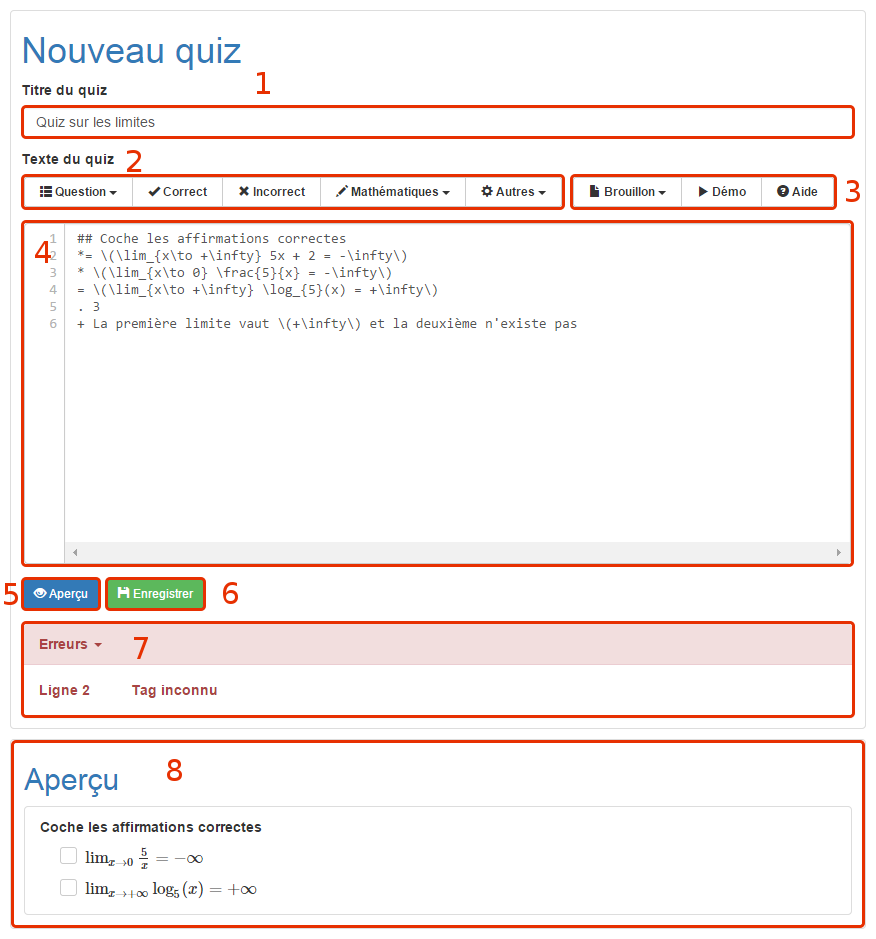
\includegraphics{create.png}
\end{figure}


\subsubsection{Création d'une question et définition de ses caractéristiques}
\label{doc-user:creation-d-une-question-et-definition-de-ses-caracteristiques}
La création du quiz se fait par l'intermédiaire d'un langage de balisage de type Markdown pour définir les différentes questions du quiz ainsi que leurs caractéristiques. Le code du quiz doit être écrit dans la zone de texte principale \textbf{(4)} La définition des questions se fait selon le schéma suivant : la première ligne du paragraphe sert à indiquer le type de question et l'énoncé, alors que les lignes suivantes décrivent les solutions ou options possibles ainsi que d'autres paramètres, comme le nombre de points attribués pour la question. Un double retour à la ligne marque le passage à la question suivante.

Au début de chaque ligne, une balise suivie d'un espace indique la fonction de la ligne en question.


\paragraph{Explication des balises}
\label{doc-user:explication-des-balises}
\begin{tabulary}{\linewidth}{|L|L|}
\hline
\textsf{\relax 
Balise
} & \textsf{\relax 
Signification
}\\
\hline
\#\#
 & 
Question à choix multiple avec plusieurs options qui peuvent être choisies
\\
\hline
**
 & 
Question à choix multiple avec une seule option qui peut être choisie
\\
\hline
??
 & 
Question avec un champ de texte à remplir
\\
\hline
*
 & 
Option invalide dans un QCM
\\
\hline
=
 & 
Option valide dans un QCM
\\
\hline
=
 & 
Réponse correcte dans une question à champ de texte
\\
\hline
.
 & 
Permet de définir le nombre de points sur la question (par défaut, 1)
\\
\hline
+
 & 
Ajout d'un commentaire d'explication qui sera affiché lors de la correction
\\
\hline\end{tabulary}



\paragraph{Exemple de quiz avec le système de balisage}
\label{doc-user:exemple-de-quiz-avec-le-systeme-de-balisage}
\begin{Verbatim}[commandchars=\\\{\}]
\PYGZsh{}\PYGZsh{} Énoncé de la question à choix multiple (plusieurs cases peuvent être cochées)
* Option 1
= Option 2 (correcte)
= Option 4 (correcte)
+ Commentaire affiché à la correction
. 1.5

** Énoncé de la question à choix multiple (une seule case peut être cochée)
* Option 1
* Option 2
= Option 3 (correcte)
. 2

?? Question à réponse courte
= Réponse correcte
= Autre réponse correcte possible
\end{Verbatim}

Pour la première question, la balise \code{\#\#} indique qu'il s'agit d'une question à choix multiple avec plusieurs réponses possibles, alors qu'une option incorrecte et deux options correctes sont respectivement définies avec les balises \code{*} et \code{=}. Ensuite, on a ajouté un commentaire avec \code{+} et défini le nombre de points avec le symbole \code{.}. Il est important de retenir que toutes les balises sont suivies d'un espace, sans quoi elles ne sont pas reconnues.

La barre d'outils située en dessus de la zone de texte offre la possibilité de créer un quiz sans maîtriser le système de balisage. Pour ajouter une question, il suffit de cliquer sur l'onglet \emph{Question} et de choisir le type de question souhaité dans le menu déroulant. La balise est insérée automatiquement et il n'y a plus qu'à écrire l'énoncé de la question. Il en va de même pour ajouter des solutions ou des options avec les boutons \emph{Correct} et \emph{Incorrect}. Les retours à la lignes et les espaces sont placés automatiquement avant et après la balise si cela est nécessaire. Le menu \emph{Autres} permet de choisir le nombre de points à attribuer pour chaque question et d'écrire un commentaire destiné à être affiché lors de la correction automatique du quiz. Ce commentaire est censé apporter une justification à la solution de la question ou une aide pour les élèves n'ayant pas répondu correctement.


\paragraph{Types de questions}
\label{doc-user:types-de-questions}

\subparagraph{Question à réponse courte}
\label{doc-user:question-a-reponse-courte}
La question à réponse courte se présente sous la forme d'un simple champ de texte à compléter. La balise caractérisant ce type de questions est la balise \code{??}. Ensuite, une ou plusieurs réponses peuvent être définies comme correctes à l'aide de la balise \code{=}. S'il y a plusieurs solutions, elles doivent être séparées par un retour à la ligne et chacune doit être précédée de la balise \code{=}. Si la réponse donné par l'élève correspond exactement à une des solutions, il obtient tous les points. Il est conseillé de ne pas définir des solutions complexes ou trop longues pour éviter de compter comme une erreur l'absence de virgule, de point ou d'un autre caractère spécial. Les réponses apportées par les élèves définies comme incorrectes lors de la correction automatique pourront toutefois être admise en tant que solution plus tard.
\begin{figure}[htbp]
\centering


\includegraphics{short.png}
\end{figure}


\subparagraph{Question à choix multiples avec un seul choix valide}
\label{doc-user:question-a-choix-multiples-avec-un-seul-choix-valide}
Pour ce type, plusieurs options sont affichées et l'élève ne peut en sélectionner qu'une. La balise associé à ce type est la balise \code{**}. Une seule option valide doit donc être définie avec la balise \code{=}, toutes les autres doivent être erronnées et donc précédées par la balise \code{*}. L'élève reçoit tous les points s'il sélectionne la bonne solution, et aucun point dans tous les autres cas.
\begin{figure}[htbp]
\centering

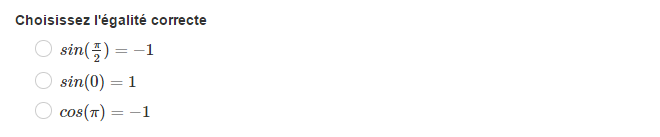
\includegraphics{radio.png}
\end{figure}


\subparagraph{Question à choix multiples avec un seul choix valide}
\label{doc-user:id1}
Définie par la balise \code{\#\#}, il s'agit d'une question semblable à la précédente mais l'élève a cette fois la possibilité de choisir plusieurs options. Les options qui doivent être sélectionnées sont définies avec la balise \code{=} et les autres avec la balise \code{*}. Le professeur doit cependant définir au moins une option correcte. Lors de la correction, l'élève peut obtenir des points pour un choix qu'il a coché et que le professeur a défini comme correct et inversément, c'est à dire qu'il peut aussi gagner des points sur un choix qui n'est pas sélectionné, à condition qu'il soit défini comme erronné.
\begin{figure}[htbp]
\centering

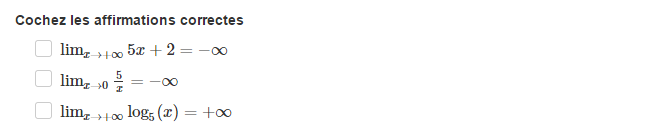
\includegraphics{checkbox.png}
\end{figure}


\subsubsection{Affichage de l'aperçu et des erreurs}
\label{doc-user:affichage-de-l-apercu-et-des-erreurs}
Il est possible à tout moment d'afficher un rendu du quiz tel que le verront les étudiants en cliquant sur le bouton \emph{Aperçu} \textbf{(5)} en dessous de la zone de texte. On peut ainsi voir si toutes les questions s'affichent comme prévu et également détecter les éventuelles erreurs dans le code. Ces erreurs apparaissent dans l'encadré rouge \textbf{(7)} en dessous du bouton \emph{Aperçu}. Pour chaque erreur, un message explicatif apparaît accompagné du numéro de ligne où s'est produite l'erreur.

Voici un exemple de code comportant une erreur :

Ici, on a tenté d'utiliser la balise \code{*=}, qui n'existe pas. C'est pourquoi on obtient le message suivant : \emph{Balise inconnue}.

Un quiz ne peut pas être envoyé et enregistré dans la base de données tant qu'il comporte encore des erreurs.


\subsubsection{Affichage de mathématiques}
\label{doc-user:affichage-de-mathematiques}
Il est possible d'afficher des formules mathématiques à l'aide de la bibliothèque Javascript MathJax. Cet outil permet d'écrire des expressions sous forme de LaTex et de les convertir en HTML pour qu'elles soient visibles dans le navigateur. Il existe deux méthodes d'affichage proposées par MathJax : la méthode \emph{in-line} et la méthode \emph{displayed}. La première méthode offre la possibilité d'inclure une formule dans un paragraphe de texte. Les formules en \emph{in-line} doivent être entourées des caractères suivants : \code{\textbackslash{}(...\textbackslash{})}. Avec la méthode \emph{displayed}, les expressions sont affichées en plus grand, centrées et détachées du reste du texte. Les formules utilisant cette méthode sont délimitées par les balises \code{\$\$...\$\$}.
\begin{figure}[htbp]
\centering

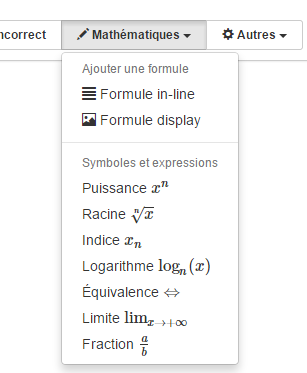
\includegraphics{math-menu.png}
\end{figure}

La barre d'outils propose un menu dédié à l'affichage des mathématiques \textbf{(2)}. Deux boutons permettent d'insérer les délimiteurs des méthodes \emph{in-line} et \emph{displayed} et d'autres options pour afficher un échantillon de formules et de symboles sont disponibles. Cette liste est toutefois non-exhaustive et il est conseillé de se référer à la documentation de LaTex {[}\#latex-doc{]} pour obtenir des informations plus précises à ce sujet.

Voici un exemple de question comportant l'affichage de limites :

\begin{Verbatim}[commandchars=\\\{\}]
\PYGZsh{}\PYGZsh{} Coche les affirmations correctes
* \PYGZbs{}(\PYGZbs{}lim\PYGZus{}\PYGZob{}x\PYGZbs{}to +\PYGZbs{}infty\PYGZcb{} 5x + 2 = \PYGZhy{}\PYGZbs{}infty\PYGZbs{})
* \PYGZbs{}(\PYGZbs{}lim\PYGZus{}\PYGZob{}x\PYGZbs{}to 0\PYGZcb{} \PYGZbs{}frac\PYGZob{}5\PYGZcb{}\PYGZob{}x\PYGZcb{} = \PYGZhy{}\PYGZbs{}infty\PYGZbs{})
= \PYGZbs{}(\PYGZbs{}lim\PYGZus{}\PYGZob{}x\PYGZbs{}to +\PYGZbs{}infty\PYGZcb{} \PYGZbs{}log\PYGZus{}\PYGZob{}5\PYGZcb{}(x) = +\PYGZbs{}infty\PYGZbs{})
\end{Verbatim}

Résultat lors de l'aperçu :
\begin{figure}[htbp]
\centering

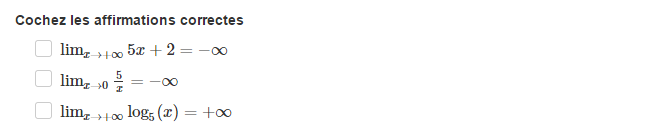
\includegraphics{checkbox.png}
\end{figure}


\subsubsection{Enregistrement et importation de brouillons}
\label{doc-user:enregistrement-et-importation-de-brouillons}
Les brouillons permettent de stocker dans la base de données le code d'un quiz qui n'a pas encore été envoyé et de le récupérer plus tard pour terminer l'édition du quiz et le publier.

Le menu \emph{Brouillons} de la barre d'outils \textbf{(3)} est dédié à cette fonctionnalité.
\begin{figure}[htbp]
\centering

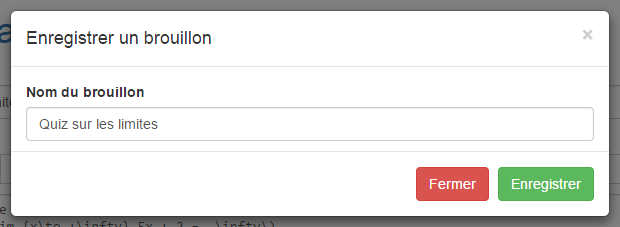
\includegraphics{draft-save.png}
\end{figure}

Lorsqu'on clique sur le bouton \emph{Enregistrer un brouillon}, une boîte de dialogue apparaît. Il suffit de préciser un titre pour le brouillon et d'appuyer sur \emph{Enregistrer}. Un message confirmant que le brouillon a bien été enregistré apparaît.
\begin{figure}[htbp]
\centering

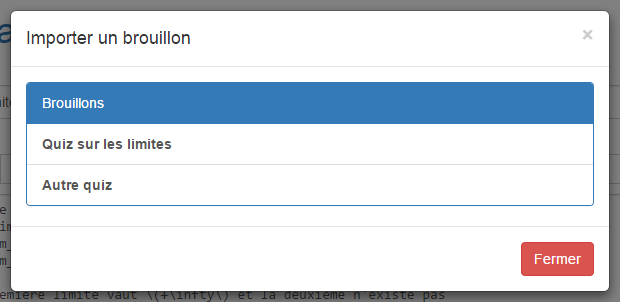
\includegraphics{draft-import.png}
\end{figure}

Il est désormais possible d'importer ce brouillon grâce au bouton prévu à cet effet dans le menu. Une boîte de dialogue contenant la liste de tous les brouillons de l'utilisateur s'ouvre. Le brouillon recherché peut être importé par un simple cliq. Le code du brouillon est alors inséré dans la zone de texte.


\subsubsection{Envoi définitif du quiz}
\label{doc-user:envoi-definitif-du-quiz}
Lorsque l'édition du quiz est terminée et que toutes les questions sont prêtes, le quiz peut être envoyé afin d'être sauvegardé dans la base de données et disponibles à la résolution pour les élèves. Avant d'envoyer un quiz, il faut s'assurer d'avoir défini un titre \textbf{(1)} et d'avoir corrigé toutes les éventuelles erreurs présentes dans le code \textbf{(7)}. Lors du cliq sur le bouton \emph{Enregistrer} \textbf{(6)}, un avertissement apparaîtra au cas où des erreurs persistent et l'envoi ne pourra pas se faire.


\subsection{Suivi des élèves}
\label{doc-user:suivi-des-eleves}

\subsubsection{Liste des quiz créés par un professeur}
\label{doc-user:liste-des-quiz-crees-par-un-professeur}\begin{figure}[htbp]
\centering

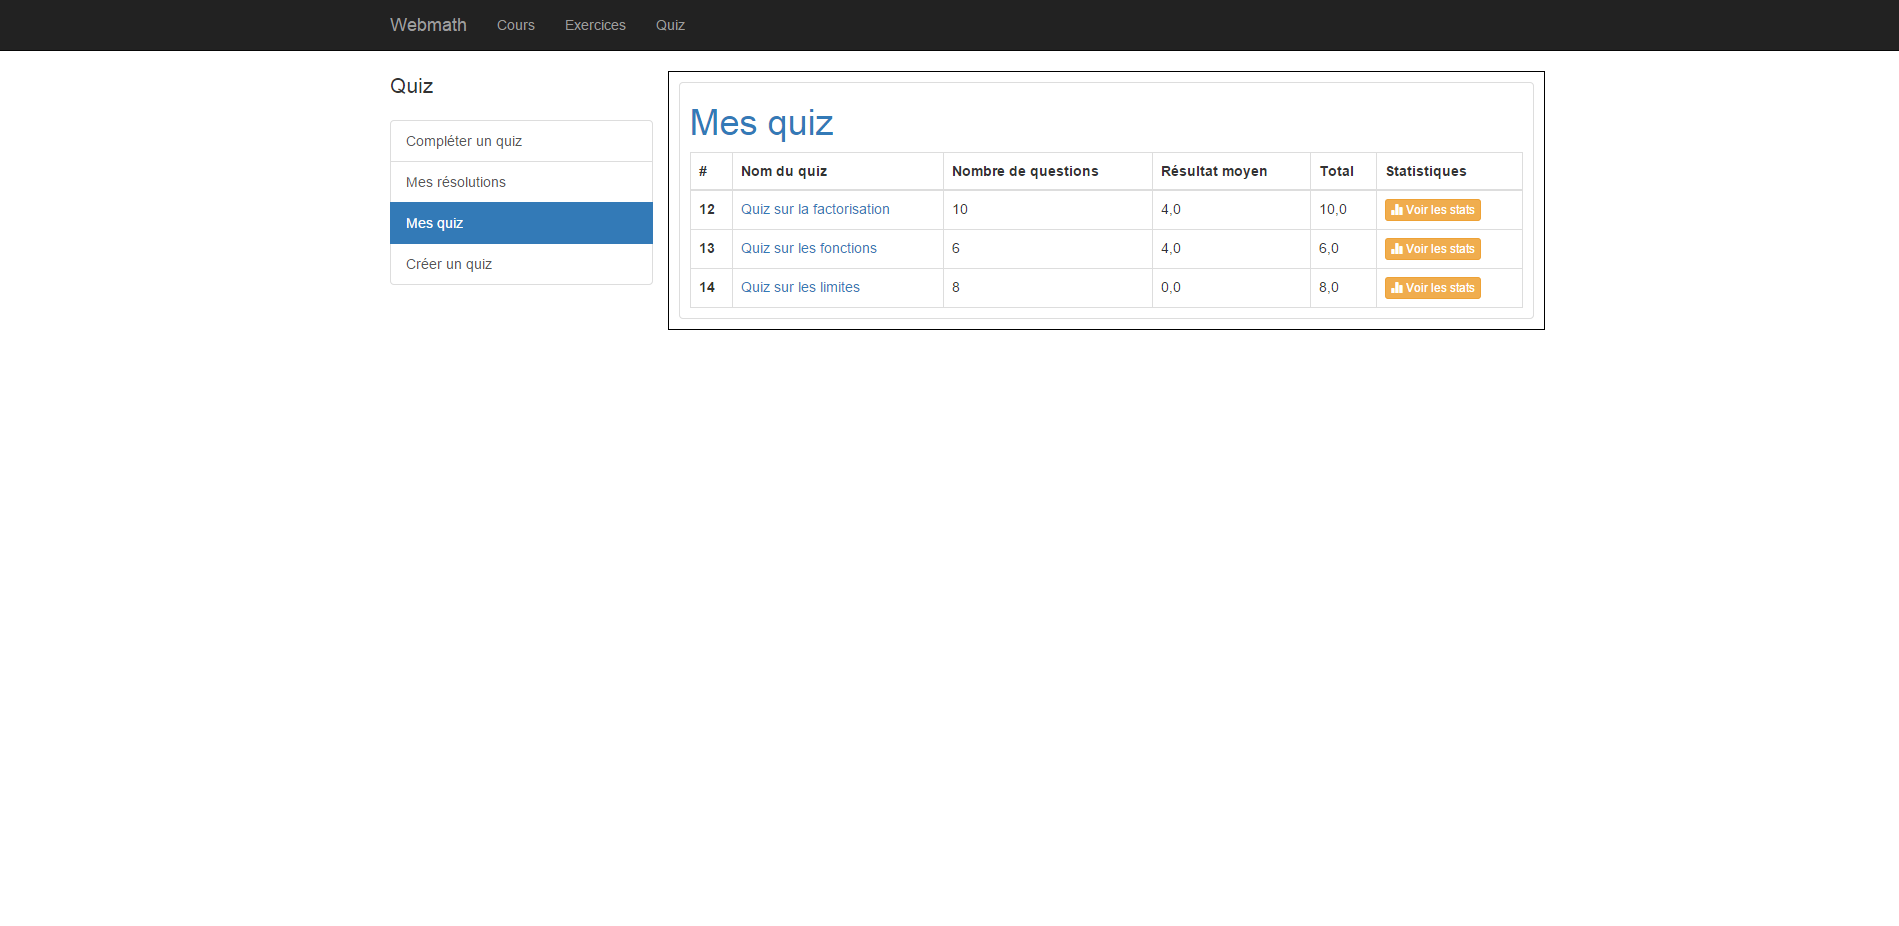
\includegraphics{my-quiz.png}
\end{figure}

Dans l'onglet \emph{Mes quiz}, le professeur peut consulter la liste des quiz qu'il a créé avec des informations générales sur ceux-ci comme la moyenne de points obtenus pour chaque quiz. Grâce au bouton \emph{Voir les stats}, il peut accéder aux statistiques avancées d'un quiz en particulier.


\subsubsection{Affichage des statistiques avancées}
\label{doc-user:affichage-des-statistiques-avancees}\begin{figure}[htbp]
\centering

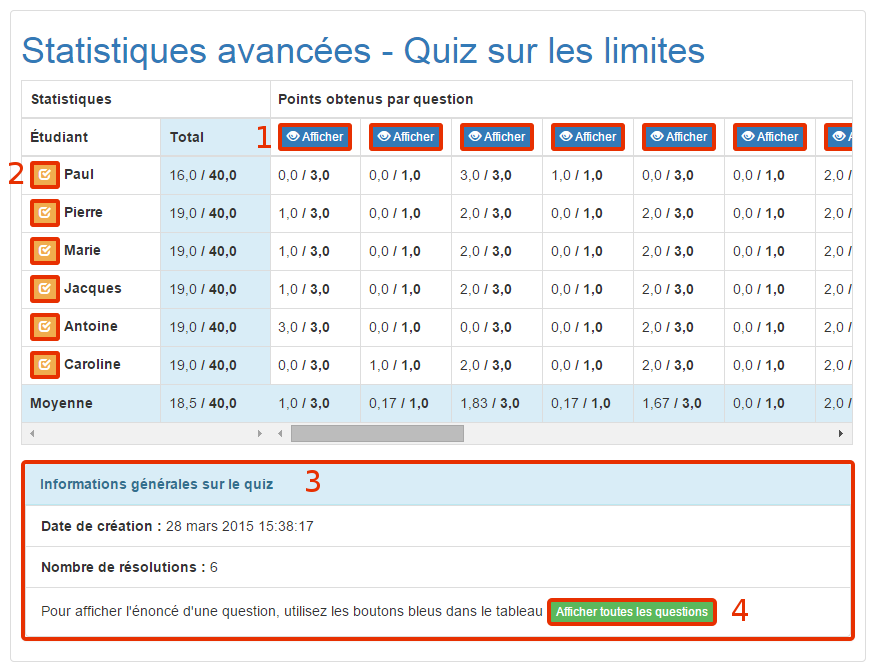
\includegraphics{stats.png}
\end{figure}

Cette vue offre au professeur la possibilité de se faire une idée générale du niveau de compréhension des élèves d'un simple coup d'oeil. Pour chaque élève ayant répondu au quiz, il peut voir la note globale obtenue ainsi que que les points attribués pour chaque question. Pour consulter les réponses soumises par un étudiant, le professeur peut cliquer sur le bouton orange situé au début de la colonne. Il sera ainsi redirigé vers la page de correction de la résolution.

Les boutons bleus \emph{Afficher} permettent de faire apparaître un aperçu rapide de chaque question. Toutes les questions du quiz peuvent aussi être consultées en même temps grâce au bouton \emph{Afficher toutes les questions}.

Lorsqu'on affiche une question à réponse courte, il est possible de voir les réponses soumises par les élèves qui n'ont pas répondu correctement. Le bouton rouge situé avant chaque réponse permet de valider une réponse et de l'ajouter aux solutions valides.
\begin{figure}[htbp]
\centering

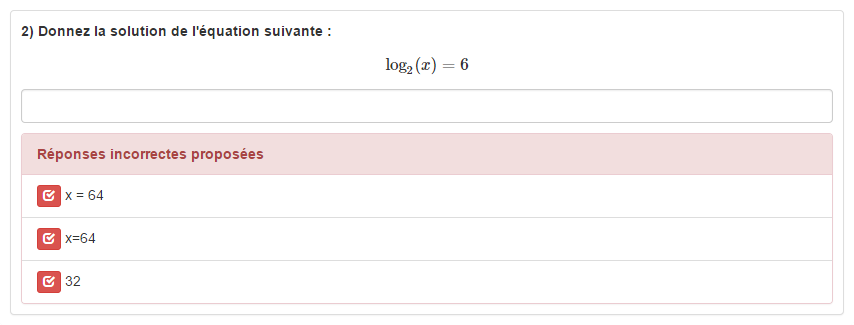
\includegraphics{add-solution.png}
\end{figure}

Ici, on voit que des étudiants ont trouvé la solution de l'équation mais l'ont simplement exprimé sous une autre forme que celle qui était attendue. Pour obtenir les points, ils auraient dû n'écrire que ``64''. Après avoir cliqué sur le bouton, un message confirmant l'ajout de la solution apparaît, puis la couleur du bouton change. Les statistiques dans le tableau se mettent ensuite à jour. Désormais, tout élève écrivant la réponse sous cette forme-là obtiendra également les points pour la question.


\section{Étudiants}
\label{doc-user:etudiants}

\subsection{Trouver un quiz}
\label{doc-user:trouver-un-quiz}\begin{figure}[htbp]
\centering

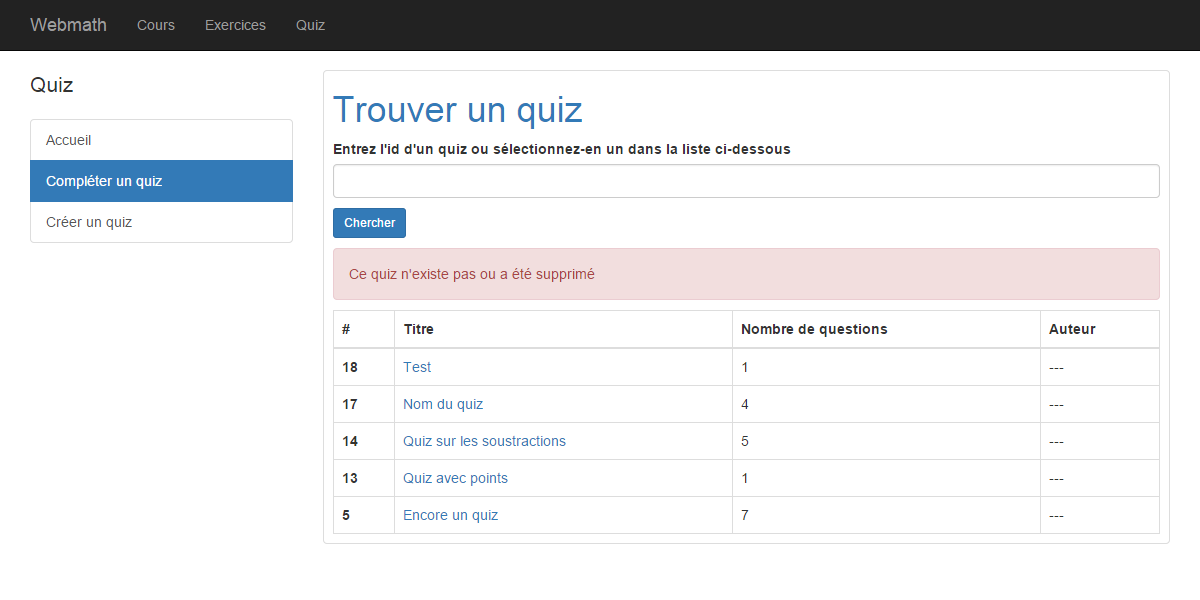
\includegraphics{find.png}
\end{figure}

Pour trouver un quiz, un étudiant a plusieurs possibilités. Le professeur peut donner l'URL exacte du quiz à compléter, ce qui peut être pratique dans le cas d'un courriel ou toute autre communicaton informatisée. Un étudiant peut aussi accéder à un quiz en mémorisant son id et en l'entrant dans la champ prévu à cet effet dans l'onglet \emph{Compléter un quiz}.


\subsection{Compléter un quiz et correction automatique}
\label{doc-user:completer-un-quiz-et-correction-automatique}\begin{figure}[htbp]
\centering

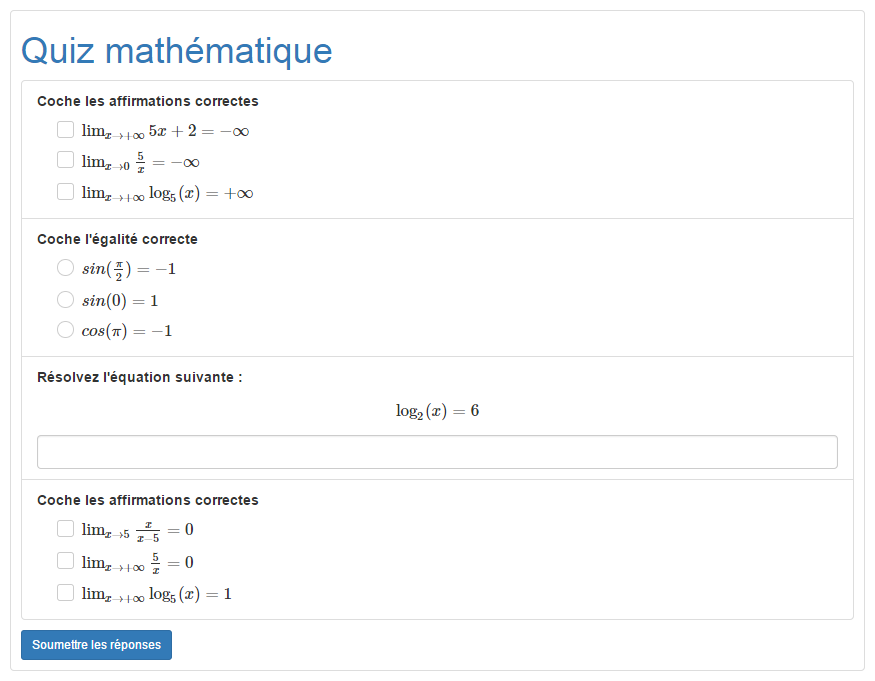
\includegraphics{complete.png}
\end{figure}

Une fois que l'étudiant à accédé au quiz, il peut le compléter très simplement en remplissant les champs de formulaires affichés. Lorsqu'il a fini, il peut soumettre ses réponses à l'aide du bouton prévu à cet effet. Les réponses soumises sont enregistrées dans la base de données et il est immédiatement redirigé vers une page de correction.

Les réponses incorrectes sont affichées en rouge avec la solution et une éventuelle explication donnée par le professeur pour chaque question. Les points reçus pour chaque question sont affichés avec le total de points sur le quiz. L'étudiant peut aussi comparer son score à la moyenne des autres étudiants qui ont complété le quiz.
\begin{figure}[htbp]
\centering

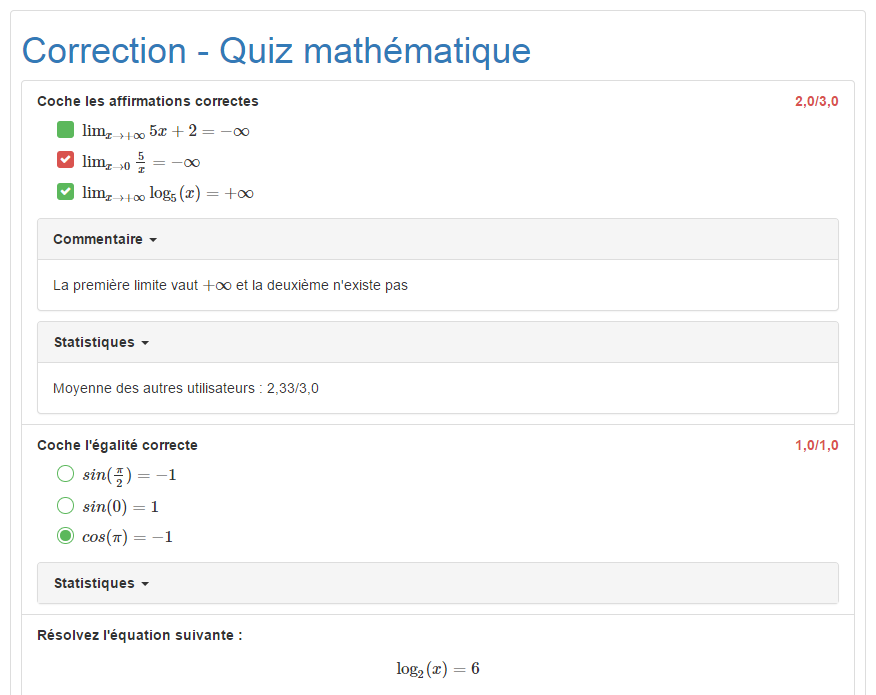
\includegraphics{correct.png}
\end{figure}

La page pour compléter un quiz ainsi que celle de la correction sont optimisées pour la navigation sur mobile et le design responsive s'adapte parfaitement à tous types de périphériques tels que les téléphones portables ou les tablettes, comme le montre la capture d'écran ci-dessous.
\begin{figure}[htbp]
\centering

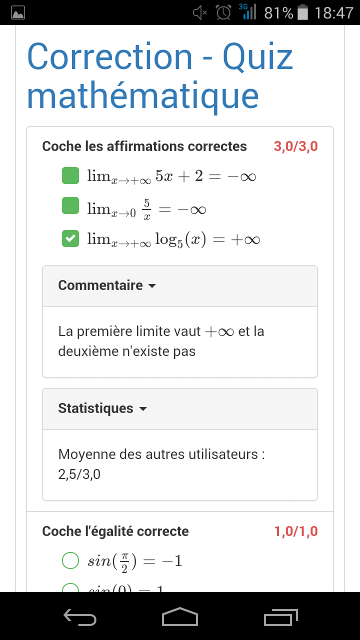
\includegraphics{mobile-1.png}
\end{figure}


\subsection{Historique des résolutions}
\label{doc-user:historique-des-resolutions}\begin{figure}[htbp]
\centering

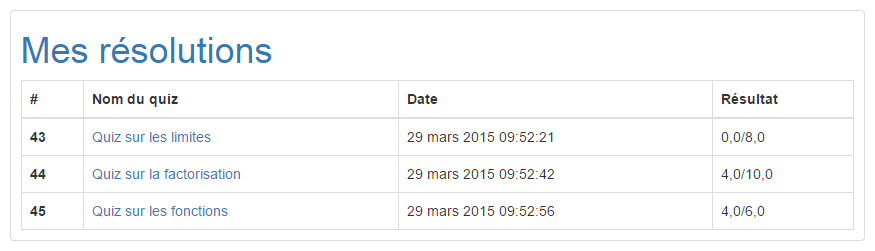
\includegraphics{completed.png}
\end{figure}

Les étudiants ont aussi la possibilité de garder une trace de tous les quiz qu'ils ont complétés. Dans l'onglet \emph{Mes résolutions} sont présentées toutes les résolutions apportées par l'élève à un quiz. Diverses informations complémentaires sont également disponibles, telles que la date et l'heure de la résolution ou le nombre de points obtenus. En cliquant sur un élément de la liste, l'étudiant est redirigé vers la page de correction de la résolution et peut ainsi voir les éventuelles erreurs qu'il a commis.


\chapter{Documentation du code source}
\label{source:documentation-du-code-source}\label{source::doc}

\section{views.py}
\label{source:views-py}\label{source:module-quiz.views}\index{quiz.views (module)}\index{add\_correct\_answer() (dans le module quiz.views)}

\begin{fulllineitems}
\phantomsection\label{source:quiz.views.add_correct_answer}\pysiglinewithargsret{\code{quiz.views.}\bfcode{add\_correct\_answer}}{\emph{request}}{}
Cette fonctionnalité donne la possibilité de définir comme correcte une réponse
soumise par l'étudiant à une question courte et de l'ajouter aux solutions de
la question en créant une nouvelle entrée dans la table \code{SqAnswer}.

Cette vue n'est utilisée que par l'intermédiaire d'une requête Ajax et n'est
accessible que si l'utilisateur est un professeur.

\textbf{Paramètres de la requête HTTP POST :}
\begin{itemize}
\item {} 
\code{answer} : Clé primaire de l'entrée dans la table \code{SqSubmit} qui doit être ajoutée aux solutions.

\end{itemize}

\end{fulllineitems}

\index{advanced\_stats() (dans le module quiz.views)}

\begin{fulllineitems}
\phantomsection\label{source:quiz.views.advanced_stats}\pysiglinewithargsret{\code{quiz.views.}\bfcode{advanced\_stats}}{\emph{request}, \emph{n\_quiz}}{}
Récupère toutes les résolutions associés au quiz avec la clé primaire \code{n\_quiz} dans la base de données et affiche
des statistiques précises montrant le résultat personnel des élèves pour chaque question.

Un objet \code{QuizForms} qui créé des formulaires Django pour toutes les question
du quiz est instancié pour permettre au professeur de visionner 
chaque question du quiz. Ce formulaire ne peut pas être envoyé et sert
uniquement à l'affichage.

\end{fulllineitems}

\index{complete() (dans le module quiz.views)}

\begin{fulllineitems}
\phantomsection\label{source:quiz.views.complete}\pysiglinewithargsret{\code{quiz.views.}\bfcode{complete}}{\emph{request}, \emph{n\_quiz}}{}
Cette vue est destinée à la résolution des quiz. Comme \code{create}, son comportement
change selon qu'il s'agisse d'une requête HTTP de type GET ou de type POST.

Dans le cas d'une requête de type GET, la vue se contente de récupérer le quiz
avec la clé primaire \code{n\_quiz} et d'instancier un objet \code{utils.submit.QuizForms} à partir
du quiz sélectionné. Cet objet prend en charge la création de tous les formulaires
Django nécessaires pour compléter le quiz (un formulaire Django par question).
Ces formulaires Django sont ensuite récupérés par l'intermédiaire de la méthode
\code{.get\_forms()} et placés dans le contexte de la fonction \code{render()}.

La requête de type POST est utilisée pour l'enregistrement des réponses soumises
au quiz par un étudiant. Là aussi, on utilise la classe \code{QuizForms}, sauf que
l'instanciation se fait avec un deuxième argument, \code{data}. Cet argument contient
en fait les données soumises par le biais des formulaires Django lorsque un
étudiant complète le quiz. Pour s'assurer de la validité de ces données, on
utilise la méthode \code{submit.QuizForms.are\_valid()} de la classe \code{QuizForms}. Une fois le
contrôle effectué, la méthode \code{.save\_answers()} se charge d'ajouter de nouvelles
entrées dans la base de donnée pour stocker les réponses soumises par l'étudiant.
Pour finir, l'utilisateur est redirigé vers la page de correction correspondant
aux réponses envoyées précédemment.

\textbf{Paramètres de la requête HTTP POST :}
\begin{itemize}
\item {} 
Ces paramètres dépendent du type et du nombre de questions qui constituent le quiz.

\end{itemize}

\end{fulllineitems}

\index{completed\_quizzes() (dans le module quiz.views)}

\begin{fulllineitems}
\phantomsection\label{source:quiz.views.completed_quizzes}\pysiglinewithargsret{\code{quiz.views.}\bfcode{completed\_quizzes}}{\emph{request}}{}
Récupère dans la base de données toutes les entrées de la table \code{CompletedQuiz}
appartenant à l'utilisateur connecté et affiche des informations générales comme
le nombre de points obtenus et un lien pour afficher la correction des réponses.

\end{fulllineitems}

\index{correct() (dans le module quiz.views)}

\begin{fulllineitems}
\phantomsection\label{source:quiz.views.correct}\pysiglinewithargsret{\code{quiz.views.}\bfcode{correct}}{\emph{request}, \emph{n\_completed}}{}
Récupère dans la base de données l'entrée de la table \code{CompletedQuiz} avec
la clé primaire \code{n\_completed} et affiche une correction détaillée des réponses soumises
par l'étudiant.

L'objet \code{CorrectQuiz} regroupe et calcule toutes les informations nécessaires
à l'affichage du quiz. Cet objet est ensuite placé dans le contexte de la fonctions
\code{render} et fournit ainsi un accès facilité aux données de la correction depuis
le template.

\end{fulllineitems}

\index{create() (dans le module quiz.views)}

\begin{fulllineitems}
\phantomsection\label{source:quiz.views.create}\pysiglinewithargsret{\code{quiz.views.}\bfcode{create}}{\emph{request}}{}
Cette vue sert à la fois à l'affichage de l'outil de création de quiz et à
l'enregistrement de nouveaux quiz.

S'il s'agit d'une requête HTTP GET, elle renvoie simplement le template de
création de quiz contenant un formulaire vide.

Au contraire, s'il la requête HTTP est de type POST, la vue se charge d'enregistrer
le nouveau quiz dans la base de données en instanciant un objet de la classe
{\hyperref[source:quiz.utils.save.SaveQuiz]{\emph{\code{utils.save.SaveQuiz}}}} avec en argument les paramètres de la requête HTTP et le compte
utilisateur du créateur du quiz. Cette
classe se charge ensuite de créer les entrées nécessaires dans les différentes tables de
la base de données.

Une fois le quiz enregistré, la vue redirige l'utilisateur vers la page de
résolution du quiz qui vient d'être créé.

\textbf{Paramètres de la requête HTTP POST :}
\begin{itemize}
\item {} 
\code{title} : Le titre du quiz

\item {} 
\code{json} : Les données des questions du quiz structurées sous forme de json. Le json sera ensuite parsé par la classe \code{SaveQuiz}.

\item {} 
\code{quizcode} : Le format texte du quiz, interprété côté client pour construire le json

\end{itemize}

\end{fulllineitems}

\index{created\_quizzes() (dans le module quiz.views)}

\begin{fulllineitems}
\phantomsection\label{source:quiz.views.created_quizzes}\pysiglinewithargsret{\code{quiz.views.}\bfcode{created\_quizzes}}{\emph{request}}{}
Récupère dans la base de données toutes les entrées de la table \code{Quiz} créées
par le professeur connecté. Les données des quiz sont utilisées pour afficher
le résultat moyen des étudiants pour le quiz, la date de création ainsi qu'un lien vers la page de
résolution du quiz ou vers les statistiques avancées.

\end{fulllineitems}

\index{find() (dans le module quiz.views)}

\begin{fulllineitems}
\phantomsection\label{source:quiz.views.find}\pysiglinewithargsret{\code{quiz.views.}\bfcode{find}}{\emph{request}}{}
Récupère dans la base de données les derniers quiz créés par des professeurs
et renvoie un template contenant des informations générales sur ces quiz et
un lien pour y accéder.

\end{fulllineitems}

\index{findquiz() (dans le module quiz.views)}

\begin{fulllineitems}
\phantomsection\label{source:quiz.views.findquiz}\pysiglinewithargsret{\code{quiz.views.}\bfcode{findquiz}}{\emph{request}}{}
Renvoie sous forme de json le titre et l'url pour accéder au quiz dont la clé primaire est donnée
en paramètre de la requête GET.

L'url du quiz est construite à l'aide de la méthode \code{reverse(vue, arguments)}
fournie par Django.
Le premier argument de la fonction \code{reverse()} est une chaîne de caractère composée du nom de l'application Django
et du nom de la vue (dans les urls) respectant le schéma suivant :
\code{"nom\_app:nom\_vue"}. L'argument \code{args} est une liste contenant les arguments
de l'URL de la page souhaitée. Ici, il s'agit simplement de la clé primaire du quiz recherché.

Cette vue est essentiellement destinée à être utilisé par une requête Ajax
depuis la vue \code{find}.

\textbf{Exemple de json renvoyé par la vue :}

\begin{Verbatim}[commandchars=\\\{\}]
\PYG{p}{\PYGZob{}}
    \PYG{n+nt}{\PYGZdq{}title\PYGZdq{}}\PYG{p}{:} \PYG{l+s+s2}{\PYGZdq{}Un quiz sympathique\PYGZdq{}}\PYG{p}{,}
    \PYG{n+nt}{\PYGZdq{}url\PYGZdq{}}\PYG{p}{:} \PYG{l+s+s2}{\PYGZdq{}/quiz/1/complete/\PYGZdq{}}
\PYG{p}{\PYGZcb{}}
\end{Verbatim}

\textbf{Paramètres de la requête HTTP GET :}
\begin{itemize}
\item {} 
\code{quiz} : Clé primaire du quiz recherché

\end{itemize}

\end{fulllineitems}

\index{getdraft() (dans le module quiz.views)}

\begin{fulllineitems}
\phantomsection\label{source:quiz.views.getdraft}\pysiglinewithargsret{\code{quiz.views.}\bfcode{getdraft}}{\emph{request}}{}
Renvoie sous forme de json le titre et le code correspondant au brouillon en
paramètre.

Cette vue est essentiellement destinée à être utilisé par une requête Ajax.

\textbf{Exemple de données d'un brouillon en json :}

\begin{Verbatim}[commandchars=\\\{\}]
\PYG{p}{\PYGZob{}}
    \PYG{n+nt}{\PYGZdq{}title\PYGZdq{}}\PYG{p}{:} \PYG{l+s+s2}{\PYGZdq{}Brouillon 1\PYGZdq{}}\PYG{p}{,}
    \PYG{n+nt}{\PYGZdq{}code\PYGZdq{}}\PYG{p}{:} \PYG{l+s+s2}{\PYGZdq{}\PYGZsh{}\PYGZsh{} Cases à cocher\PYGZbs{}n * Option 1\PYGZbs{}n= Option 4\PYGZbs{}n= Option 5\PYGZdq{}}
\PYG{p}{\PYGZcb{}}
\end{Verbatim}

\textbf{Paramètres de la requête HTTP GET :}
\begin{itemize}
\item {} 
\code{draft} : Clé primaire du brouillon

\end{itemize}

\end{fulllineitems}

\index{listdrafts() (dans le module quiz.views)}

\begin{fulllineitems}
\phantomsection\label{source:quiz.views.listdrafts}\pysiglinewithargsret{\code{quiz.views.}\bfcode{listdrafts}}{\emph{request}}{}
Renvoie le titre et la clé primaire de tous les brouillons de l'utilisateur connecté
sous forme de json.

\textbf{Exemple de json renvoyé dans le cas d'un professeur ayant
enregistré deux brouillons :}

\begin{Verbatim}[commandchars=\\\{\}]
\PYG{p}{[}
    \PYG{p}{\PYGZob{}}
        \PYG{n+nt}{\PYGZdq{}title\PYGZdq{}}\PYG{p}{:} \PYG{l+s+s2}{\PYGZdq{}Brouillon 1\PYGZdq{}}\PYG{p}{,}
        \PYG{n+nt}{\PYGZdq{}id\PYGZdq{}}\PYG{p}{:} \PYG{l+m+mi}{1}
    \PYG{p}{\PYGZcb{}}\PYG{p}{,}
    \PYG{p}{\PYGZob{}}
        \PYG{n+nt}{\PYGZdq{}title\PYGZdq{}}\PYG{p}{:} \PYG{l+s+s2}{\PYGZdq{}Brouillon 2\PYGZdq{}}\PYG{p}{,}
        \PYG{n+nt}{\PYGZdq{}id\PYGZdq{}}\PYG{p}{:} \PYG{l+m+mi}{2}
    \PYG{p}{\PYGZcb{}}
\PYG{p}{]}
\end{Verbatim}

Cette vue est essentiellement destinée à être utilisé par requête Ajax.

\end{fulllineitems}

\index{savedraft() (dans le module quiz.views)}

\begin{fulllineitems}
\phantomsection\label{source:quiz.views.savedraft}\pysiglinewithargsret{\code{quiz.views.}\bfcode{savedraft}}{\emph{request}}{}
Créé une nouvelle entrée dans la table \code{QuizDraft}. Le brouillon est associé
à l'utilisateur connecté et enregistre les valeurs données en paramètres pour
les colonnes \code{title} et \code{code}.

Cette vue n'est disponible que si l'utilisateur connecté appartient au groupe
`teachers'.

\textbf{Paramètres de la requête HTTP POST :}
\begin{itemize}
\item {} 
\code{title} : Titre du brouillon

\item {} 
\code{code} : Code du quiz

\end{itemize}

\end{fulllineitems}



\section{models.py}
\label{source:module-quiz.models}\label{source:models-py}\index{quiz.models (module)}\index{CompletedQuiz (classe dans quiz.models)}

\begin{fulllineitems}
\phantomsection\label{source:quiz.models.CompletedQuiz}\pysiglinewithargsret{\strong{class }\code{quiz.models.}\bfcode{CompletedQuiz}}{\emph{*args}, \emph{**kwargs}}{}
Contient
\index{get\_questions\_submits() (méthode quiz.models.CompletedQuiz)}

\begin{fulllineitems}
\phantomsection\label{source:quiz.models.CompletedQuiz.get_questions_submits}\pysiglinewithargsret{\bfcode{get\_questions\_submits}}{}{}
Renvoie la liste des entrées des tables \code{SqSubmit}, \code{QcmSubmitOne} et
\code{QcmSubmitMulti} correspondant à la résolution \code{self}.
Chaque élément de cette liste représente concrètement la réponse soumise à
une question du quiz.

Cette liste est triée selon l'ordre d'apparition des questions correspondant
réponses proposées.

\end{fulllineitems}

\index{update\_total\_result() (méthode quiz.models.CompletedQuiz)}

\begin{fulllineitems}
\phantomsection\label{source:quiz.models.CompletedQuiz.update_total_result}\pysiglinewithargsret{\bfcode{update\_total\_result}}{}{}
Met à jour le nombre de points obtenus pour la résolution du quiz en entier
en fonction des points obtenus pour chaque réponse soumise aux questions
du quiz.

Pour comptabiliser le nombre total de points obtenus, cette méthode parcourt
la liste des réponses apportées avec la méthode {\hyperref[source:quiz.models.CompletedQuiz.get_questions_submits]{\emph{\code{CompletedQuiz.get\_questions\_submits()}}}}
appliquée à la résolution en question.
calcule la somme des points obtenus pour chacune des questions.

Cette méthode peut être utilisée lorsqu'une résolution vient d'être soumise
par un élève pour comptabiliser une première fois les points obtenus ou 
lorsqu'une entrée dans {\hyperref[source:quiz.models.SqAnswer]{\emph{\code{SqAnswer}}}} a été ajoutée pour mettre à jour les
statistques en fonction des changements.

\end{fulllineitems}


\end{fulllineitems}

\index{Qcm (classe dans quiz.models)}

\begin{fulllineitems}
\phantomsection\label{source:quiz.models.Qcm}\pysiglinewithargsret{\strong{class }\code{quiz.models.}\bfcode{Qcm}}{\emph{id}, \emph{text}, \emph{comment}, \emph{points}, \emph{number}, \emph{id\_quiz\_id}, \emph{multi\_answers}}{}~\index{average\_result() (méthode quiz.models.Qcm)}

\begin{fulllineitems}
\phantomsection\label{source:quiz.models.Qcm.average_result}\pysiglinewithargsret{\bfcode{average\_result}}{}{}
Récupère toutes les réponses soumises pour la question et renvoie la moyenne
arrondie à deux chiffres après la virgule sur la base du nombre de réponses
proposées et sur la somme des résultats obtenus.

\end{fulllineitems}

\index{create\_form() (méthode quiz.models.Qcm)}

\begin{fulllineitems}
\phantomsection\label{source:quiz.models.Qcm.create_form}\pysiglinewithargsret{\bfcode{create\_form}}{\emph{*args}, \emph{**kwargs}}{}
Retourne un formulaire Django permettant à un étudiant de répondre à la question
\code{self}. Le formulaire sera de type \code{RadioForm} si un seul choix
peut être sélectionné et de type \code{CheckboxForm} si la question autorise
l'étudiant à cocher plusieurs options.

Les arguments fournis lors de l'instanciation du formulaire sont analogues
à ceux qui sont donnés pour l'instanciation d'un \code{TextForm} dans {\hyperref[source:quiz.models.SimpleQuestion.create_form]{\emph{\code{SimpleQuestion.create\_form()}}}}.

\end{fulllineitems}

\index{save\_submit() (méthode quiz.models.Qcm)}

\begin{fulllineitems}
\phantomsection\label{source:quiz.models.Qcm.save_submit}\pysiglinewithargsret{\bfcode{save\_submit}}{\emph{data}, \emph{completed}}{}
Enregistre une nouvelle entrée dans la table {\hyperref[source:quiz.models.QcmSubmitMulti]{\emph{\code{QcmSubmitMulti}}}}
ou {\hyperref[source:quiz.models.QcmSubmitOne]{\emph{\code{QcmSubmitOne}}}} selon qu'il s'agisse d'une question avec
plusieurs options correctes ou une seule. Ces tables permettent de stocker
le(s) choix sélectionné(s) par l'étudiant pour la question \code{self}.

La récupération des données du formulaire à partir de l'argument \code{data}
et l'instanciation du modèle est analogue à la manipulation effectuée dans {\hyperref[source:quiz.models.SimpleQuestion.save_submit]{\emph{\code{SimpleQuestion.save\_submit()}}}}

\end{fulllineitems}


\end{fulllineitems}

\index{QcmChoice (classe dans quiz.models)}

\begin{fulllineitems}
\phantomsection\label{source:quiz.models.QcmChoice}\pysiglinewithargsret{\strong{class }\code{quiz.models.}\bfcode{QcmChoice}}{\emph{id}, \emph{text}, \emph{valid}, \emph{id\_question\_id}}{}~\index{checked() (méthode quiz.models.QcmChoice)}

\begin{fulllineitems}
\phantomsection\label{source:quiz.models.QcmChoice.checked}\pysiglinewithargsret{\bfcode{checked}}{\emph{qcmsubmit}}{}
Détermine si le choix a été sélectionné ou non dans la réponse soumise
\code{qcmsubmit}.

S'il la question peut admettre plusieurs options correctes, deux conditions doivent
être remplies. D'abord, au moins un choix doit avoir été coché dans \code{qcmsubmit}.
Cette vérification est nécessaire car le champ \code{qcmsubmit.id\_selected} peut
valoir \code{null} dans la base de données. Ensuite, il suffit de regarder
si le choix se trouve dans la liste des options sélectionnés avec la méthode
\code{qcmsubmit.id\_selected.all()}.

Dans le cas d'une question avec une seule réponse correcte, la méthode
vérifie simplement que l'élément sélectionné corresponde au choix défini comme
correct.

\end{fulllineitems}

\index{correct\_submit() (méthode quiz.models.QcmChoice)}

\begin{fulllineitems}
\phantomsection\label{source:quiz.models.QcmChoice.correct_submit}\pysiglinewithargsret{\bfcode{correct\_submit}}{\emph{qcmsubmit}}{}
Détermine le choix \code{self} a été coché correctement dans la réponse
soumise \code{qcmsubmit}. Si l'option a été cochée et qu'elle est définie
comme valide, la méthode renvoie \code{True}. Si l'option est cochée mais
définie comme invalide, la valeur de retour sera cette fois \code{False}.
Si l'élève n'a pas coché l'option, le raisonnement se fera de manière analogue
mais dans le sens inverse.

\end{fulllineitems}


\end{fulllineitems}

\index{QcmSubmitMulti (classe dans quiz.models)}

\begin{fulllineitems}
\phantomsection\label{source:quiz.models.QcmSubmitMulti}\pysiglinewithargsret{\strong{class }\code{quiz.models.}\bfcode{QcmSubmitMulti}}{\emph{id}, \emph{result}, \emph{id\_submitted\_quiz\_id}, \emph{id\_question\_id}}{}~\index{save\_result() (méthode quiz.models.QcmSubmitMulti)}

\begin{fulllineitems}
\phantomsection\label{source:quiz.models.QcmSubmitMulti.save_result}\pysiglinewithargsret{\bfcode{save\_result}}{}{}
Comptabilise et enregistre les points obtenus par rapport aux choix cochés.

Cette méthode parcourt tous les choix possibles pour la question
\code{self.id\_question} récupérés avec \code{Qcm.get\_choices()}. Pour chaque
choix, elle utilise la méthode {\hyperref[source:quiz.models.QcmChoice.correct_submit]{\emph{\code{QcmChoice.correct\_submit()}}}} pour
vérifier que le choix a été coché correctement. L'étudiant obtient une part
des points pour chaque choix correct.

\end{fulllineitems}


\end{fulllineitems}

\index{QcmSubmitOne (classe dans quiz.models)}

\begin{fulllineitems}
\phantomsection\label{source:quiz.models.QcmSubmitOne}\pysiglinewithargsret{\strong{class }\code{quiz.models.}\bfcode{QcmSubmitOne}}{\emph{id}, \emph{result}, \emph{id\_submitted\_quiz\_id}, \emph{id\_question\_id}, \emph{id\_selected\_id}}{}~\index{save\_result() (méthode quiz.models.QcmSubmitOne)}

\begin{fulllineitems}
\phantomsection\label{source:quiz.models.QcmSubmitOne.save_result}\pysiglinewithargsret{\bfcode{save\_result}}{}{}
Comptabilise et enregistre les points obtenus par raport au choix sélectionné.

Si le choix sélectionné correspond à la solution, tous les points sont attribués.
Si aucune option n'est choisie, l'étudiant obtient automatiquement zéro point.

\end{fulllineitems}


\end{fulllineitems}

\index{Quiz (classe dans quiz.models)}

\begin{fulllineitems}
\phantomsection\label{source:quiz.models.Quiz}\pysiglinewithargsret{\strong{class }\code{quiz.models.}\bfcode{Quiz}}{\emph{*args}, \emph{**kwargs}}{}
Table dont le rôle est de stocker les informations générales sur le quiz telles
que le titre du quiz, le nombre maximal de points pouvant être obtenus ou la date
et l'heure de sa création.

Tous les modèles contenant les données des questions du quiz incluent une clé
étrangère reliant la question avec la table \code{{}`Quiz}.
\index{average\_result() (méthode quiz.models.Quiz)}

\begin{fulllineitems}
\phantomsection\label{source:quiz.models.Quiz.average_result}\pysiglinewithargsret{\bfcode{average\_result}}{}{}
Récupère dans la base de données toutes les résolutions se rattachant
au quiz en question puis calcule la moyenne des résultats obtenus sur la base
du résultat de chaque élève et le nombre de résolutions envoyées.

\end{fulllineitems}

\index{get\_questions() (méthode quiz.models.Quiz)}

\begin{fulllineitems}
\phantomsection\label{source:quiz.models.Quiz.get_questions}\pysiglinewithargsret{\bfcode{get\_questions}}{}{}
Récupère la liste de toutes les questions du quiz et les trie dans l'ordre
d'apparition dans le quiz.

\end{fulllineitems}

\index{length() (méthode quiz.models.Quiz)}

\begin{fulllineitems}
\phantomsection\label{source:quiz.models.Quiz.length}\pysiglinewithargsret{\bfcode{length}}{}{}
Retourne le nombre de questions qui composent le quiz.

\end{fulllineitems}


\end{fulllineitems}

\index{QuizDraft (classe dans quiz.models)}

\begin{fulllineitems}
\phantomsection\label{source:quiz.models.QuizDraft}\pysiglinewithargsret{\strong{class }\code{quiz.models.}\bfcode{QuizDraft}}{\emph{*args}, \emph{**kwargs}}{}
La table \code{QuizDraft} sert à stocker les brouillons. Elle contient le titre
du brouillon, le code ainsi qu'une relation vers le créateur du brouillon.

\end{fulllineitems}

\index{SimpleQuestion (classe dans quiz.models)}

\begin{fulllineitems}
\phantomsection\label{source:quiz.models.SimpleQuestion}\pysiglinewithargsret{\strong{class }\code{quiz.models.}\bfcode{SimpleQuestion}}{\emph{id}, \emph{text}, \emph{comment}, \emph{points}, \emph{number}, \emph{id\_quiz\_id}}{}~\index{average\_result() (méthode quiz.models.SimpleQuestion)}

\begin{fulllineitems}
\phantomsection\label{source:quiz.models.SimpleQuestion.average_result}\pysiglinewithargsret{\bfcode{average\_result}}{}{}
Renvoie le nombre moyen de points obtenus pour la question en se basant sur
le nombre total de réponses soumises et sur la somme de tous les points obtenus.
La moyenne est ensuite arrondie à deux chiffres après la virgule pour éviter
tout problème d'affichage.

Au cas où aucune réponse n'a encore été soumise, cette méthode retourne
simplement la chaîne \code{-{-}} qui peut directement être utilisée dans le template.

\end{fulllineitems}

\index{create\_form() (méthode quiz.models.SimpleQuestion)}

\begin{fulllineitems}
\phantomsection\label{source:quiz.models.SimpleQuestion.create_form}\pysiglinewithargsret{\bfcode{create\_form}}{\emph{*args}, \emph{**kwargs}}{}
Instancie un formulaire Django personnalisé de type \code{TextForm} correspondant
à la question. Ce type de formulaire est défini dans py:mod:\emph{forms} et spécialement
conçu pour les questions à réponse courte.

Lors de l'instanciation, plusieurs arguments sont fournis. Premièrement,
on indique la question \code{self} pour que des informations supplémentaires
la concernant puissent éventuellement être obtenues depuis le formulaire.CompletedQuiz
Ensuite, l'index de la position de la question dans le quiz est attribué à
l'argument \code{prefix}. Cet argument permet d'identifier la question correspondant
au formulaire lorsque les données entrées par l'utilisateur sont récupérées.

\end{fulllineitems}

\index{get\_wrong\_answers() (méthode quiz.models.SimpleQuestion)}

\begin{fulllineitems}
\phantomsection\label{source:quiz.models.SimpleQuestion.get_wrong_answers}\pysiglinewithargsret{\bfcode{get\_wrong\_answers}}{}{}
Retourne la liste de toutes les réponses incorrectes soumises pour la question \code{self}.
Pour éviter les doublons, les réponses équivalentes sont renvoyées une seule fois.
Par exemple, si deux réponses valent \code{"5"}, seule la première sera renvoyée par
cette méthode.

Comme cette méthode est utilisée pour afficher les réponses soumises incorrectes pouvant
potentiellement être définies comme correctes par la suite au cas où le 
professeur les juge acceptables, les réponses vides sont aussi exclues 
puisqu'il n'y aurait pas de sens à les admettre dans les solutions.

\end{fulllineitems}

\index{save\_submit() (méthode quiz.models.SimpleQuestion)}

\begin{fulllineitems}
\phantomsection\label{source:quiz.models.SimpleQuestion.save_submit}\pysiglinewithargsret{\bfcode{save\_submit}}{\emph{data}, \emph{completed}}{}
Cette méthode permet d'enregistrer dans la base de données une réponse soumise
par l'utilisateur à la question \code{self} en créant une entrée dans la table
\code{SqSubmit}.

L'argument \code{data} est dictionnaire contenant les paramètres de la 
requête HTTP qui concernent le formulaire créé pour la question. On peut donc
facilement accéder au texte entré par l'élève avec la clé \code{'answer'}.

L'argument \code{completed} contient la référence vers l'élément de la table
\code{CompletedQuiz} qui comprend les données de la résolution de l'élève. On
peut ainsi facilement relier l'entrée créée dans \code{SqSubmit} avec la résolution
de l'élève.

\end{fulllineitems}

\index{update\_question\_results() (méthode quiz.models.SimpleQuestion)}

\begin{fulllineitems}
\phantomsection\label{source:quiz.models.SimpleQuestion.update_question_results}\pysiglinewithargsret{\bfcode{update\_question\_results}}{}{}
Permet de réévaluer toutes les réponses soumises pour la question après
l'ajout d'une solution correcte pour corriger les statistiques.

Pour ceci, la méthode récupère la liste des réponses soumises à la question
dans la table \code{SqSubmit}. Elle applique la méthode \code{.save\_result} à 
chacune d'entre elles. De plus,
comme le résultat de la résolution peut changer, il faut aussi mettre à jour
le résultat total obtenu pour la résolution (table \code{CompletedQuiz}) liée à chaque réponse soumise.

\end{fulllineitems}


\end{fulllineitems}

\index{SqAnswer (classe dans quiz.models)}

\begin{fulllineitems}
\phantomsection\label{source:quiz.models.SqAnswer}\pysiglinewithargsret{\strong{class }\code{quiz.models.}\bfcode{SqAnswer}}{\emph{id}, \emph{text}, \emph{id\_question\_id}}{}
\end{fulllineitems}

\index{SqSubmit (classe dans quiz.models)}

\begin{fulllineitems}
\phantomsection\label{source:quiz.models.SqSubmit}\pysiglinewithargsret{\strong{class }\code{quiz.models.}\bfcode{SqSubmit}}{\emph{id}, \emph{text}, \emph{result}, \emph{id\_question\_id}, \emph{id\_submitted\_quiz\_id}}{}~\index{build\_correct() (méthode quiz.models.SqSubmit)}

\begin{fulllineitems}
\phantomsection\label{source:quiz.models.SqSubmit.build_correct}\pysiglinewithargsret{\bfcode{build\_correct}}{}{}
Instancie et retourne un objet \code{CorrectSq} correspondant à la réponse soumise \code{self}.
La classe :py:class:\code{CorrectSq} permet un accès plus rapide aux données nécessaires à
l'affichage de la correction.

\end{fulllineitems}

\index{correct() (méthode quiz.models.SqSubmit)}

\begin{fulllineitems}
\phantomsection\label{source:quiz.models.SqSubmit.correct}\pysiglinewithargsret{\bfcode{correct}}{}{}
Détermine si la réponse soumise est correcte en vérifiant qu'elle se
se trouve dans la liste des solutions correctes.

\end{fulllineitems}

\index{get\_corrections() (méthode quiz.models.SqSubmit)}

\begin{fulllineitems}
\phantomsection\label{source:quiz.models.SqSubmit.get_corrections}\pysiglinewithargsret{\bfcode{get\_corrections}}{}{}
Renvoie la liste des solutions correctes pour la question sous forme de liste de
chaînes de charactères

\end{fulllineitems}

\index{save\_result() (méthode quiz.models.SqSubmit)}

\begin{fulllineitems}
\phantomsection\label{source:quiz.models.SqSubmit.save_result}\pysiglinewithargsret{\bfcode{save\_result}}{}{}
Comptabilise et enregistre les points obtenus pour la réponse soumise. Si la réponse soumise
est correcte, tous les points sont attribués. Dans le cas contraire,
aucun point n'est attribué.

\end{fulllineitems}

\index{set\_as\_correct() (méthode quiz.models.SqSubmit)}

\begin{fulllineitems}
\phantomsection\label{source:quiz.models.SqSubmit.set_as_correct}\pysiglinewithargsret{\bfcode{set\_as\_correct}}{}{}
Si la réponse soumise à la question avait été définie comme incorrecte
lors de la correction automatique, cette méthode permet d'ajouter la réponse
soumise aux solutions correctes de la question.

Toutes les réponses soumises pour la question sont ensuite réeavaluées pour
mettre à jour les statistiques.

\end{fulllineitems}


\end{fulllineitems}



\section{forms.py}
\label{source:forms-py}\label{source:module-quiz.forms}\index{quiz.forms (module)}\index{CheckboxForm (classe dans quiz.forms)}

\begin{fulllineitems}
\phantomsection\label{source:quiz.forms.CheckboxForm}\pysiglinewithargsret{\strong{class }\code{quiz.forms.}\bfcode{CheckboxForm}}{\emph{queryset}, \emph{*args}, \emph{**kwargs}}{}
Formulaire Django personnalisé correspondant à une question à choix multiples
pouvant admettre plusieurs réponses correctes.

Le type de champ de formulaire utilisé est un \code{ModelMultipleChoiceField}. Ce champ permet
de sélectionner plusieurs entrées d'une table de la base de données par l'intermédiaire
de cases à cocher. Ici, il s'agit
de la table :py:class{}`models.QcmChoice{}`.

L'argument \code{queryset} permet de définir les choix qui seront affichés, il s'agit
d'une liste d'entrées de la table :py:class{}`models.QcmChoice{}`.
\index{get\_type() (méthode quiz.forms.CheckboxForm)}

\begin{fulllineitems}
\phantomsection\label{source:quiz.forms.CheckboxForm.get_type}\pysiglinewithargsret{\bfcode{get\_type}}{}{}
Retourne \code{1} pour donner une indication sur la manière d'afficher 
la question dans le template

\end{fulllineitems}


\end{fulllineitems}

\index{QuestionForm (classe dans quiz.forms)}

\begin{fulllineitems}
\phantomsection\label{source:quiz.forms.QuestionForm}\pysiglinewithargsret{\strong{class }\code{quiz.forms.}\bfcode{QuestionForm}}{\emph{question}, \emph{*args}, \emph{**kwargs}}{}
Classe abstraite dont héritent tous les formulaires destinés à la résolution
des quiz. Seul l'attribut \code{question} est défini. Il correspond à la référence
de la question dans la base de données et permet d'afficher facilement des informations
sur la question depuis le template.

\end{fulllineitems}

\index{RadioForm (classe dans quiz.forms)}

\begin{fulllineitems}
\phantomsection\label{source:quiz.forms.RadioForm}\pysiglinewithargsret{\strong{class }\code{quiz.forms.}\bfcode{RadioForm}}{\emph{queryset}, \emph{*args}, \emph{**kwargs}}{}
Formulaire Django personnalisé correspondant à une question à choix multiples
avec une seule réponse correcte.

Ici, on utilise un champ de formulaire \code{ModelChoiceField}. Il s'agit du même principe
que pour {\hyperref[source:quiz.forms.CheckboxForm]{\emph{\code{CheckboxForm}}}} sauf qu'un seul choix peut être sélectionné et
que le formulaire est affiché en HTML sous forme de boutons radio.
\index{get\_type() (méthode quiz.forms.RadioForm)}

\begin{fulllineitems}
\phantomsection\label{source:quiz.forms.RadioForm.get_type}\pysiglinewithargsret{\bfcode{get\_type}}{}{}
Retourne \code{1} pour donner une indication sur la manière d'afficher 
la question dans le template

\end{fulllineitems}


\end{fulllineitems}

\index{TextForm (classe dans quiz.forms)}

\begin{fulllineitems}
\phantomsection\label{source:quiz.forms.TextForm}\pysiglinewithargsret{\strong{class }\code{quiz.forms.}\bfcode{TextForm}}{\emph{*args}, \emph{**kwargs}}{}
Formulaire Django personnalisé destiné à l'affichage des questions à réponse courte.

Un \code{CharField} constitue l'unique champ de ce formulaire. Il s'agit simplement
d'un champ de texte basique dans lequel l'étudiant peut écrire sa réponse.
\index{get\_type() (méthode quiz.forms.TextForm)}

\begin{fulllineitems}
\phantomsection\label{source:quiz.forms.TextForm.get_type}\pysiglinewithargsret{\bfcode{get\_type}}{}{}
Retourne \code{0} pour donner une indication sur la manière d'afficher 
la question dans le template

\end{fulllineitems}


\end{fulllineitems}



\section{utils/submit.py}
\label{source:module-quiz.utils.submit}\label{source:utils-submit-py}\index{quiz.utils.submit (module)}\index{QuizForms (classe dans quiz.utils.submit)}

\begin{fulllineitems}
\phantomsection\label{source:quiz.utils.submit.QuizForms}\pysiglinewithargsret{\strong{class }\code{quiz.utils.submit.}\bfcode{QuizForms}}{\emph{quiz}, \emph{data=None}}{}
Le rôle de cette classe est de créer des formulaires Django correspondant aux
questions d'un quiz en particulier puis de fournir des méthodes pour traiter
les données récupérées grâce aux formulaires et de les enregistrer.
\index{are\_valid() (méthode quiz.utils.submit.QuizForms)}

\begin{fulllineitems}
\phantomsection\label{source:quiz.utils.submit.QuizForms.are_valid}\pysiglinewithargsret{\bfcode{are\_valid}}{}{}
Applique la méthode \code{.is\_valid()} à chaque formulaire correspondant à une
question et renvoie \code{True} si aucun problème survient avec la validation.

\end{fulllineitems}

\index{save\_answers() (méthode quiz.utils.submit.QuizForms)}

\begin{fulllineitems}
\phantomsection\label{source:quiz.utils.submit.QuizForms.save_answers}\pysiglinewithargsret{\bfcode{save\_answers}}{\emph{user}}{}
Cette méthode permet de sauvegarder dans la base de données les réponses
soumises par le biais des formulaires Django correspondant à chaque question.

Pour ce faire, une nouvelle entrée dans la table \code{CompletedQuiz} est
d'abord créée. Ensuite, la méthode parcourt parallèlement la liste des questions
du quiz et les formulaires correspondants. Pour chaque question, elle appelle
la méthode \code{.save\_submit()} avec en argument les données récupérées à partir
du formulaire associé à la question. La méthode \code{.save\_submit()} se charge
de sauvegarder les données concernant les réponses soumises aux différentes
questions. La manière de traiter ces données dépendera du type de question
dont il s'agit. On peut appliquer la méthode \code{.save\_submit()} à chacune
des questions du quiz sans se soucier du type car son comportement est défini
différement selon la classe à laquelle appartient la question.

\end{fulllineitems}


\end{fulllineitems}



\section{utils/correct.py}
\label{source:utils-correct-py}\label{source:module-quiz.utils.correct}\index{quiz.utils.correct (module)}
Ensemble d'objets pour permettre un accès facilité aux données nécessaires à
l'affichage des corrections
\index{CorrectChoice (classe dans quiz.utils.correct)}

\begin{fulllineitems}
\phantomsection\label{source:quiz.utils.correct.CorrectChoice}\pysiglinewithargsret{\strong{class }\code{quiz.utils.correct.}\bfcode{CorrectChoice}}{\emph{choice}, \emph{qcmsubmit}}{}
Fournis des raccourcis pour accéder aux données des choix de QCM à corriger.
Cette classe permet d'indiquer le texte à afficher avec le choix, de déterminer
s'il a été coché et s'il est correct.

\end{fulllineitems}

\index{CorrectQcm (classe dans quiz.utils.correct)}

\begin{fulllineitems}
\phantomsection\label{source:quiz.utils.correct.CorrectQcm}\pysiglinewithargsret{\strong{class }\code{quiz.utils.correct.}\bfcode{CorrectQcm}}{\emph{qcmsubmit}}{}
Facilite l'affichage de la correction des questions à choix multiples par
l'intermédiaire de raccourcis et instancie des objets de type {\hyperref[source:quiz.utils.correct.CorrectChoice]{\emph{\code{CorrectChoice}}}}.

L'attribut \code{type} vaut \code{1} pour les QCM à réponses multiples, \code{2} pour
les listes déroulantes et \code{3} pour les QCM à réponse unique.

\end{fulllineitems}

\index{CorrectQuestion (classe dans quiz.utils.correct)}

\begin{fulllineitems}
\phantomsection\label{source:quiz.utils.correct.CorrectQuestion}\pysiglinewithargsret{\strong{class }\code{quiz.utils.correct.}\bfcode{CorrectQuestion}}{\emph{submit}}{}
Définit des raccourcis pour accéder aux attributs communs à tous les types
de questions.

\end{fulllineitems}

\index{CorrectSq (classe dans quiz.utils.correct)}

\begin{fulllineitems}
\phantomsection\label{source:quiz.utils.correct.CorrectSq}\pysiglinewithargsret{\strong{class }\code{quiz.utils.correct.}\bfcode{CorrectSq}}{\emph{sqsubmit}}{}
Fournit des attributs spécifiques à la correction des questions à réponse courte.
L'attribut \code{type} permet d'identifier dans le template le type de question
dont il s'agit et de déterminer la manière d'afficher la correction.

Pour une question à réponse courte, \code{type} vaut \code{0}.

\end{fulllineitems}



\section{utils/save.py}
\label{source:module-quiz.utils.save}\label{source:utils-save-py}\index{quiz.utils.save (module)}\index{SaveQcm (classe dans quiz.utils.save)}

\begin{fulllineitems}
\phantomsection\label{source:quiz.utils.save.SaveQcm}\pysiglinewithargsret{\strong{class }\code{quiz.utils.save.}\bfcode{SaveQcm}}{\emph{question}, \emph{*args}, \emph{**kwargs}}{}
Enregistre une question à choix multiples dans la base de données. S'il s'agit
d'une question à réponses correctes multiples, il faut assigner la valeur \code{True}
à l'attribut \code{multi\_answers}. Par défaut, celui-ci reçoit la valeur \code{False}.
Les différentes options à sélectionner sont également enregistrées.
\index{add\_option() (méthode quiz.utils.save.SaveQcm)}

\begin{fulllineitems}
\phantomsection\label{source:quiz.utils.save.SaveQcm.add_option}\pysiglinewithargsret{\bfcode{add\_option}}{\emph{option}}{}
Ajoute une option à la question en créant une nouvelle entrée dans la table
\code{models.QcmChoice}.

\end{fulllineitems}


\end{fulllineitems}

\index{SaveQuestion (classe dans quiz.utils.save)}

\begin{fulllineitems}
\phantomsection\label{source:quiz.utils.save.SaveQuestion}\pysiglinewithargsret{\strong{class }\code{quiz.utils.save.}\bfcode{SaveQuestion}}{\emph{question}, \emph{Model}, \emph{quiz\_db}, \emph{n}}{}
Classe abstraite qui créé une nouvelle question dans la base de données avec
les attributs communs à tous les types de questions. La méthode \code{.save()}
n'est pas encore utilisée car certains attributs doivent encore être ajoutés
dans les classes filles.

La table concernée peut être \code{models.SimpleQuestion} ou \code{models.Qcm}.
Cela dépend de l'argument \code{Model} qui définit la classe à utiliser.

L'argument \code{question} est un dictionnaire contenant les données sur la question.
Les arguments \emph{quiz\_db{}`} et \code{n} correspondent respectivement à la référence
du quiz dans la table :py:class:models.Quiz{}`{}` et à l'index de la position
de la question.

\end{fulllineitems}

\index{SaveQuiz (classe dans quiz.utils.save)}

\begin{fulllineitems}
\phantomsection\label{source:quiz.utils.save.SaveQuiz}\pysiglinewithargsret{\strong{class }\code{quiz.utils.save.}\bfcode{SaveQuiz}}{\emph{title}, \emph{questions\_list}, \emph{quizcode}, \emph{teacher}}{}
Classe permettant l'enregistrement d'un quiz et de toutes ses questions dans
la base de données. Une première entrée \code{models.Quiz} est enregistrée
puis les données des questions sont sauvegardées par l'intermédiaire des classes
{\hyperref[source:quiz.utils.save.SaveSimpleQuestion]{\emph{\code{SaveSimpleQuestion}}}} et {\hyperref[source:quiz.utils.save.SaveQcm]{\emph{\code{SaveQcm}}}}.

\end{fulllineitems}

\index{SaveSimpleQuestion (classe dans quiz.utils.save)}

\begin{fulllineitems}
\phantomsection\label{source:quiz.utils.save.SaveSimpleQuestion}\pysiglinewithargsret{\strong{class }\code{quiz.utils.save.}\bfcode{SaveSimpleQuestion}}{\emph{question}, \emph{*args}, \emph{**kwargs}}{}
Enregistre une question à réponse courte dans la base de données. Tous les champs
de la base de données ont déjà été définis par {\hyperref[source:quiz.utils.save.SaveQuestion]{\emph{\code{SaveQuestion}}}},
la méthode \code{.save()} peut donc être utilisée directement. Les différentes
solutions sont ensuite sauvegardées.
\index{add\_answer() (méthode quiz.utils.save.SaveSimpleQuestion)}

\begin{fulllineitems}
\phantomsection\label{source:quiz.utils.save.SaveSimpleQuestion.add_answer}\pysiglinewithargsret{\bfcode{add\_answer}}{\emph{text}}{}
Ajoute une solution à la question en créant un champ dans la table 
\code{models.SqAnswer}

\end{fulllineitems}


\end{fulllineitems}



\chapter{Modèle relationnel}
\label{database:modele-relationnel}\label{database::doc}

\section{Introduction}
\label{database:introduction}
Une des premières étapes importantes dans le développement d'un site web est l'élaboration d'un modèle relationnel structuré permettant de stocker toutes les données générées par l'application et de les relier entre elles. Un modèle relationnel décrit les différentes tables de la base de données et les liens entre ces tables. Une table peut être comparée à un tableau contenant des informations. Chaque table comporte une ou plusieurs colonnes, chaque colonne stockant un type de données précisément défini, par exemple un nombre entier ou une chaîne de caractères. Si on imagine une table contenant les données sur les utilisateurs d'un site, une colonne pourrait alors contenir le pseudonyme d'un utilisateur et une autre son âge. On peut ensuite ajouter des entrées dans une table, c'est à dire un ensemble de données dont chaque élément correspond à une colonne de la table. Dans l'exemple précédent, on ajouterait ainsi une ligne pour chaque utilisateur s'inscrivant sur le site. Chaque ligne est identifiée grâce à une clé primaire unique, habituellement sous la forme d'un entier, qui permet de créer des liens entre différentes lignes de différentes tables. Ces liens entre différentes tables sont appelées relations.

Voici, présenté sous forme simplifiée à l'aide d'un tableau, comment on pourrait stocker les données concernant des quiz et leurs créateurs :

\textbf{Table contenant les utilisateurs :}

\begin{tabulary}{\linewidth}{|L|L|L|}
\hline
\textsf{\relax 
Clé primaire
} & \textsf{\relax 
Prénom
} & \textsf{\relax 
Âge
}\\
\hline
1
 & 
Paul
 & 
26
\\
\hline
2
 & 
Juliette
 & 
22
\\
\hline
3
 & 
Marc
 & 
48
\\
\hline\end{tabulary}


\textbf{Table contenant les quiz :}

\begin{tabulary}{\linewidth}{|L|L|L|}
\hline
\textsf{\relax 
Clé primaire
} & \textsf{\relax 
Titre du quiz
} & \textsf{\relax 
Auteur
}\\
\hline
1
 & 
Fonctions exponentielles
 & 
3
\\
\hline
2
 & 
Logarithmes
 & 
3
\\
\hline
3
 & 
Comportement à l'infini
 & 
2
\\
\hline\end{tabulary}


Ici, le premier quiz a comme titre \emph{Fonctions exponentielles}, comporte 5 questions et a été créé par Marc (Utilisateur 3).

Une fois que le modèle relationnel a été élaboré, on peut créer une base de données sous forme de fichier. Le langage SQL permet de créer les tables d'une base de données, d'y enregistrer des informations et de faire des requêtes, c'est à dire récupérer des données enregistrées. Un logiciel ou une application web peut ainsi communiquer avec une base de données et stocker les informations nécessaires de manière permanente.

Django offre la possibilité de créer une base de données et d'interagir avec celle-ci par le biais d'une ORM (Object Relational Mapper), on peut donc éviter l'utilisation du langage SQL et communiquer avec la base de données avec des objets et des méthodes Python. Cet aspect de Django sera abordé un peu plus loin.


\section{Utilisation dans l'application de création de quiz}
\label{database:utilisation-dans-l-application-de-creation-de-quiz}

\subsection{Implémentation dans Django}
\label{database:implementation-dans-django}
Comme indiqué précédemment, Django fournit une interface de haut niveau pour créer et interagir avec une base de données. On peut écrire nos tables avec une architecture orientée objet, que Django ``traduira'' ensuite en SQL. Ainsi, pour créer une table dans notre base de données, il suffit de définir une classe héritant de \code{models.Model} et d'initialiser des variables de classes pour ajouter des colonnes à la tables. Ainsi, par exemple, pour implémenter une table contenant les données générales d'un quiz, il suffit d'écrire le code suivant :

\begin{Verbatim}[commandchars=\\\{\}]
\PYG{k}{class} \PYG{n+nc}{Quiz}\PYG{p}{(}\PYG{n}{models}\PYG{o}{.}\PYG{n}{Model}\PYG{p}{)}\PYG{p}{:} \PYG{c}{\PYGZsh{}Infos générales sur le quiz}
    \PYG{n}{title} \PYG{o}{=} \PYG{n}{models}\PYG{o}{.}\PYG{n}{CharField}\PYG{p}{(}\PYG{n}{max\PYGZus{}length}\PYG{o}{=}\PYG{l+m+mi}{100}\PYG{p}{)} \PYG{c}{\PYGZsh{}Colonne contenant une chaîne de caractères}
    \PYG{n}{creation\PYGZus{}date} \PYG{o}{=} \PYG{n}{models}\PYG{o}{.}\PYG{n}{DateTimeField}\PYG{p}{(}\PYG{p}{)} \PYG{c}{\PYGZsh{}Colonne contenant une date/heure}
    \PYG{n}{code} \PYG{o}{=} \PYG{n}{models}\PYG{o}{.}\PYG{n}{CharField}\PYG{p}{(}\PYG{n}{max\PYGZus{}length}\PYG{o}{=}\PYG{l+m+mi}{1000}\PYG{p}{)} \PYG{c}{\PYGZsh{}Colonne contenant une chaîne de caractères}
\end{Verbatim}

Les objets comme \code{CharField()} ou \code{DateTimeField()} permettent de définir des champs d'un type de données précis. Une liste complète des types de champs est disponible sur la documentation officielle de Django : \href{https://docs.djangoproject.com/en/1.7/ref/models/fields/\#field-types}{https://docs.djangoproject.com/en/1.7/ref/models/fields/\#field-types}


\subsection{Schéma global}
\label{database:schema-global}
L'élaboration d'un schéma relationnel n'est pas chose facile car il est nécessaire que celui ci réponde à certains critères. Il doit être relativement simple afin de garder une certaine flexibilité et d'avoir la possiblité d'être modifié plus tard, car il est souvent difficile de prédire à l'avance les difficultés liées au stockage des données qui pourraient être rencontrées au cours du développement. Il doit également être possible d'ajouter des fonctionnalités sans devoir revoir toute l'organisation du schéma ou créer un trop grand nombre de nouvelles tables. Malgré cela, le modèle doit aussi correspondre aux exigences des fonctionnalités de l'application et doit inclure toutes les relations nécessaires. Il s'agit donc d'une étape cruciale qui peut s'avérer décisive pour la suite du développement.

Voici le diagramme des tables utilisés pour stocker les données des quiz :
\begin{figure}[htbp]
\centering

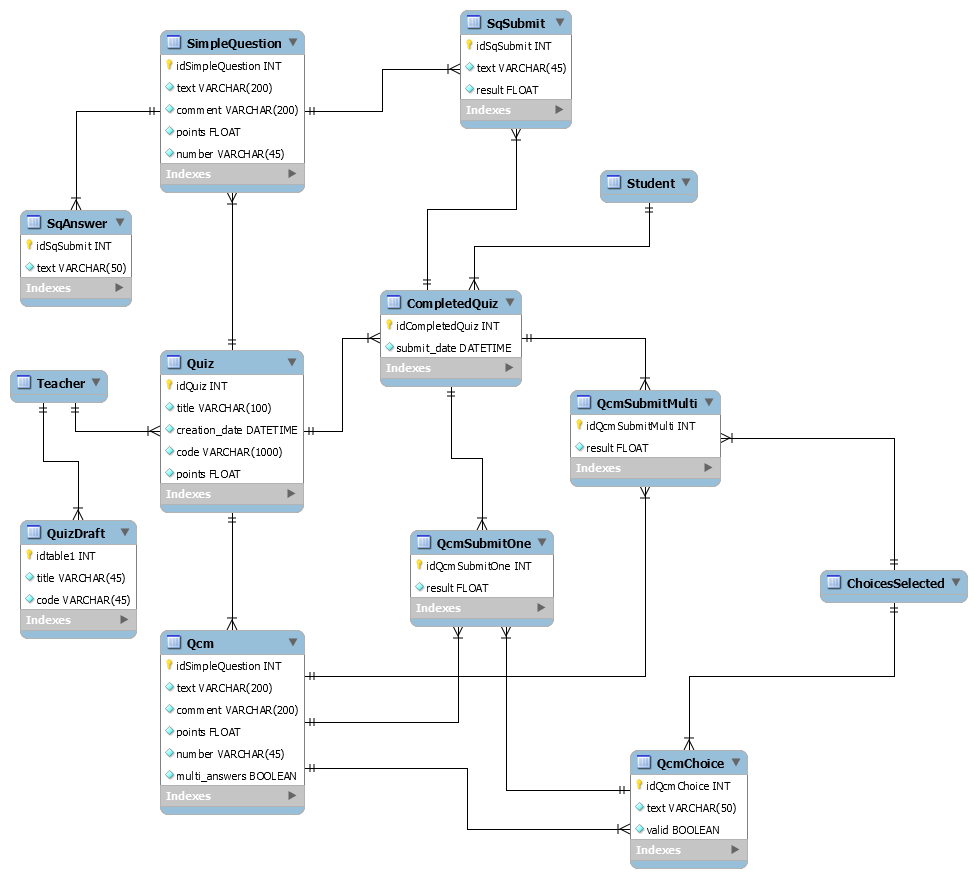
\includegraphics{quiz-models.png}
\end{figure}


\subsection{Explications des tables}
\label{database:explications-des-tables}

\subsubsection{\texttt{Quiz}}
\label{database:quiz}
La table \code{Quiz} est la table centrale de l'application et toutes les autres tables s'organisent autour d'elle. Elle comporte trois colonnes importantes : une contenant le titre, une autre contenant la date et l'heure de création (ajouté automatiquement lorsqu'un nouveau quiz est créé) ainsi qu'une colonne dans laquelle est stockée le nombre maximal de points pouvant être obtenus pour le quiz en question. Cette table comporte également une relation vers une table Teacher  qui permet l'intégration dans le projet de groupe.

Avec django, il est possible d'initialiser automatiquement un champ \code{DateTimeField} à la date/heure du moment où le modèle est instancié avec le paramètre \code{auto\_now\_add}

\begin{Verbatim}[commandchars=\\\{\}]
\PYG{n}{creation\PYGZus{}date} \PYG{o}{=} \PYG{n}{models}\PYG{o}{.}\PYG{n}{DateTimeField}\PYG{p}{(}\PYG{n}{auto\PYGZus{}now\PYGZus{}add}\PYG{o}{=}\PYG{n+nb+bp}{True}\PYG{p}{)}
\end{Verbatim}


\subsubsection{\texttt{QuizDraft}}
\label{database:quizdraft}
Cette table est un peu isolée dans le schéma relationnel et n'a qu'une fonction : enregistrer le code qu'un quiz qu'un professeur n'a pas terminé et lui offrir la possibilité de le récupérer plus tard pour continuer son travail. Outre la relation vers la table \code{Teacher} et la colonne stockant le code du quiz, une colonne permet de stocker un titre pour pouvoir identifier rapidement un brouillon.


\subsubsection{\texttt{SimpleQuestion}}
\label{database:simplequestion}
Cette table contient les informations générales sur les questions simples du quiz. Ces questions sont présentées sous la forme d'un simple champ de texte lorsqu'un élève complète le quiz. Une première colonne \code{title} stocke l'énoncé de la question, \code{comment} permet d'inclure un commentaire affiché lors de la correction automatique du quiz (par exemple la démonstration d'une égalité), \code{points} définit le nombre de points attribués sur cette question et \code{number} enregistre l'ordre auquel doit apparaître la question dans le quiz. Une relation désigne le quiz qui intègre la question.


\subsubsection{\texttt{SqAnswer}}
\label{database:sqanswer}
Cette table contient simplement la solution de la question définie par la relation vers la table \emph{SimpleQuestion}. Il est important de noter qu'il peut y avoir plusieurs solutions possibles pour une question et c'est la raison pour laquelle la solution n'est pas simplement stockée dans une colonne de \emph{SimpleQuestion}.


\subsubsection{\texttt{Qcm}}
\label{database:qcm}
La table Qcm permet de stocker les informations générales à propos des questions à choix multiples. Ces questions sont affichées sous forme de boutons radio, de cases à cocher ou de liste déroulante.
Cette table reprend plusieurs colonnes de la table \emph{SimpleQuestion}. C'est pourquoi ces deux tables héritent en fait du même modèle dans django :

\begin{Verbatim}[commandchars=\\\{\}]
\PYG{k}{class} \PYG{n+nc}{QuizQuestion}\PYG{p}{(}\PYG{n}{models}\PYG{o}{.}\PYG{n}{Model}\PYG{p}{)}\PYG{p}{:} \PYG{c}{\PYGZsh{}Classe abstraite dont héritent toutes les questions}
    \PYG{n}{text} \PYG{o}{=} \PYG{n}{models}\PYG{o}{.}\PYG{n}{CharField}\PYG{p}{(}\PYG{n}{max\PYGZus{}length}\PYG{o}{=}\PYG{l+m+mi}{200}\PYG{p}{)} \PYG{c}{\PYGZsh{}Énoncé}
    \PYG{n}{comment} \PYG{o}{=} \PYG{n}{models}\PYG{o}{.}\PYG{n}{CharField}\PYG{p}{(}\PYG{n}{max\PYGZus{}length}\PYG{o}{=}\PYG{l+m+mi}{200}\PYG{p}{,} \PYG{n}{blank}\PYG{o}{=}\PYG{n+nb+bp}{True}\PYG{p}{)} \PYG{c}{\PYGZsh{}Commentaire}
    \PYG{n}{points} \PYG{o}{=} \PYG{n}{models}\PYG{o}{.}\PYG{n}{FloatField}\PYG{p}{(}\PYG{n}{default}\PYG{o}{=}\PYG{l+m+mi}{1}\PYG{p}{)}
    \PYG{n}{number} \PYG{o}{=} \PYG{n}{models}\PYG{o}{.}\PYG{n}{IntegerField}\PYG{p}{(}\PYG{p}{)} \PYG{c}{\PYGZsh{}Ordre de la question dans le quiz}
    \PYG{n}{id\PYGZus{}quiz} \PYG{o}{=} \PYG{n}{models}\PYG{o}{.}\PYG{n}{ForeignKey}\PYG{p}{(}\PYG{n}{Quiz}\PYG{p}{)}

    \PYG{k}{class} \PYG{n+nc}{Meta}\PYG{p}{:}
        \PYG{n}{abstract} \PYG{o}{=} \PYG{n+nb+bp}{True}

\PYG{k}{class} \PYG{n+nc}{SimpleQuestion}\PYG{p}{(}\PYG{n}{QuizQuestion}\PYG{p}{)}\PYG{p}{:}
    \PYG{k}{pass} \PYG{c}{\PYGZsh{}Cette table reprend simplement les mêmes colonnes que le modèle abstrait}

\PYG{k}{class} \PYG{n+nc}{Qcm}\PYG{p}{(}\PYG{n}{QuizQuestion}\PYG{p}{)}\PYG{p}{:}
    \PYG{n}{multi\PYGZus{}answers} \PYG{o}{=} \PYG{n}{models}\PYG{o}{.}\PYG{n}{BooleanField}\PYG{p}{(}\PYG{p}{)}
\end{Verbatim}

En plus des colonnes héritées de \code{QuizQuestion{}`}, \code{Qcm} possède un champ de type booléen. Il s'agit de \code{multi\_answers}, qui détermine si plusieurs options peuvent êres cochées ou non. Si ce champ vaut \code{True}, la question sera affiché sous forme de cases à cocher en HTML. Dans le cas contraire, elle sera affichée à l'aide de boutons radio.


\subsubsection{\texttt{QcmChoice}}
\label{database:qcmchoice}
Cette table contient les différents choix possibles pour la question définie par la relation vers \code{Qcm}. Elle est formée de deux champs, le premier contenant le texte du choix et l'autre définissant par un booléen s'il est correct ou non de cocher ce choix. Une question à choix multiples doit avoir au moins deux choix possibles et au moins un choix correct. Si \code{multi\_answers} vaut \code{False} dans \code{Qcm}, une seule option peut être correcte puisque l'étudiant n'a la possibilité de cocher qu'une seule option.

\textbf{Note :} D'un point de vue purement relationnel, comme il est indiqué sur le diagramme, cette table possède une relation vers une table qui sert d'intermédiaire entre \emph{QcmChoice} et \code{QcmSubmitMulti}. Cette table intermédiaire crée en fait une relation de type \emph{Complexe-Complexe}. L'implémentation de ce type de relation avec Django sera abordé plus loin.


\subsubsection{\texttt{CompletedQuiz}}
\label{database:completedquiz}
Comme on peut le voir sur le diagramme, à l'instar de \code{Quiz}, cette table occupe aussi un rôle central dans le modèle relationnel. Elle permet de faire le lien entre un quiz créé par un professeur et les réponses soumises à ce quiz par les étudiants. Elle possède donc une relation vers une table \code{Student}, qui définit l'étudiant ayant répondu au quiz. De l'autre côté, cette table pointe vers \code{Quiz} et définit logiquement le quiz auquel l'étudiant a répondu. Un seul champ est présent : la date et l'heure de la soumission des réponses.


\subsubsection{\texttt{SqSubmit}}
\label{database:sqsubmit}
Il s'agit simplement de la réponse apportée à une question simple. La table a donc un champ \code{text} qui contient la réponse soumise par l'élève et un champ \code{result} qui stocke le nombre de points obtenus pour la question. Elle possède aussi deux relations, une vers \code{SimpleQuestion} pour préciser la question auquel l'élève a répondu, et une autre vers \emph{CompletedQuiz}. La réponse soumise par l'élève sera ensuite comparée à(aux) solution(s) enregistrées pour déterminer si les points sont attribués ou non.


\subsubsection{\texttt{QcmSubmitOne et QcmSubmitMulti}}
\label{database:qcmsubmitone-et-qcmsubmitmulti}
Ces deux tables sont très similaires. \code{QcmSubmitOne} contient une relation vers l'option sélectionnée par l'étudiant dans une question à choix multiples avec \emph{multi\_answers} valant \code{False{}`}, tandis que \code{QcmSubmitMulti} peut contenir des relations vers plusieurs options, quand \code{multi\_answers} vaut \code{True}. Il s'agit donc dans le premier cas d'une relation \emph{Complexe-Simple}, puique plusieurs lignes peuvent pointer vers la même option. Dans le deuxième cas, c'est une relation de type \emph{Complexe-Complexe}, puisque plusieurs lignes peuvent pointer vers plusieurs options.

Dans Django, voici comment seront définies ces relations :

\begin{Verbatim}[commandchars=\\\{\}]
\PYG{n}{id\PYGZus{}selected} \PYG{o}{=} \PYG{n}{models}\PYG{o}{.}\PYG{n}{ForeignKey}\PYG{p}{(}\PYG{n}{QcmChoice}\PYG{p}{,} \PYG{n}{null}\PYG{o}{=}\PYG{n+nb+bp}{True}\PYG{p}{)} \PYG{c}{\PYGZsh{}Relation Complexe\PYGZhy{}Simple}
\PYG{n}{id\PYGZus{}selected} \PYG{o}{=} \PYG{n}{models}\PYG{o}{.}\PYG{n}{ManyToManyField}\PYG{p}{(}\PYG{n}{QcmChoice}\PYG{p}{,} \PYG{n}{null}\PYG{o}{=}\PYG{n+nb+bp}{True}\PYG{p}{)} \PYG{c}{\PYGZsh{}Relation Complexe\PYGZhy{}Complexe}
\end{Verbatim}

L'argument \code{null} vaut ici \code{True} car il se peut que l'étudiant ne coche aucun choix. Dans ce cas-là, il n'obtiendra dans tous les cas aucun point.

En plus de ces relations, ces tables enregistrent aussi le nombre de points obtenus par l'étudiant pour la question dans la colonne \code{result}.


\renewcommand{\indexname}{Index des modules Python}
\begin{theindex}
\def\bigletter#1{{\Large\sffamily#1}\nopagebreak\vspace{1mm}}
\bigletter{q}
\item {\texttt{quiz.forms}}, \pageref{source:module-quiz.forms}
\item {\texttt{quiz.models}}, \pageref{source:module-quiz.models}
\item {\texttt{quiz.utils.correct}}, \pageref{source:module-quiz.utils.correct}
\item {\texttt{quiz.utils.save}}, \pageref{source:module-quiz.utils.save}
\item {\texttt{quiz.utils.submit}}, \pageref{source:module-quiz.utils.submit}
\item {\texttt{quiz.views}}, \pageref{source:module-quiz.views}
\end{theindex}

\renewcommand{\indexname}{Index}
\printindex
\end{document}
